\documentclass[11pt,a4paper]{article}
\usepackage[margin=3cm]{geometry}
\usepackage{amsmath,amssymb}
\usepackage{siunitx}          % better tables
\usepackage{booktabs}
\usepackage{graphicx}
\usepackage{hyperref}
\usepackage{caption}
\usepackage{subcaption}
\usepackage{pgfplots}         % for TikZ/PGF plots if desired
\pgfplotsset{compat=1.18}

\title{NumOps Project 3: Lasso Optimization Algorithms}
\author{Youniss Kandah\\JKU Linz}
\date{August 2025}

\begin{document}
\maketitle

\begin{abstract}
This report documents the implementation and analysis of three optimization algorithms for Lasso-type problems: Forward-Backward (FB), Projected Gradient (PG), and Active-Set Method (ASM). The project focuses on approximating the sine function over $[-2\pi, 2\pi]$ using polynomial regression while encouraging sparsity in the coefficient vector. We implement these algorithms and compare their performance on both penalized and constrained Lasso formulations, including analysis of condition numbers and pre-conditioning strategies.
\end{abstract}

\tableofcontents
\newpage

\section{Introduction}

\subsection{Development Environment}

The project is implemented in Python 3.13 using modern development tools:

\begin{itemize}
    \item \textbf{Package Manager}: UV for fast dependency resolution
    \item \textbf{Virtual Environment}: Isolated Python environment for reproducibility
    \item \textbf{Core Dependencies}: NumPy, Matplotlib, SciPy, Pandas
    \item \textbf{Development Tools}: pytest, black, flake8
\end{itemize}

\subsection{Project Structure}

The codebase is organized into modular components:

\begin{verbatim}
num_opt_proj_3/
├── src/
│   ├── algorithms/     # Optimization algorithms (FB, PG, ASM)
│   ├── problems/       # Problem formulations
│   ├── utils/          # Utility functions
│   └── experiments/    # Experiment scripts
├── results/
│   ├── plots/          # Generated plots
│   └── data/           # Numerical results
├── docs/               # Documentation and reports
├── Makefile            # Build and run commands
└── pyproject.toml      # Project configuration
\end{verbatim}

\section{Core Implementation}

\subsection{Problem Formulation}

The core problem formulation has been implemented in the \texttt{SineApproximationProblem} class. This class encapsulates:

\begin{itemize}
    \item \textbf{Vandermonde Matrix Construction}: Creates matrix $A$ where $A[j,i] = a_j^i$ for sample points $a_j$ and powers $i = 0, 1, \ldots, n$
    \item \textbf{Objective Function}: Implements $f(x) = \frac{1}{2}\|Ax - b\|_2^2$ with gradient $\nabla f(x) = A^\top(Ax - b)$ and Hessian $\nabla^2 f(x) = A^\top A$
    \item \textbf{Problem Properties}: Computes Lipschitz constant $L = \|A^\top A\|_2$ and condition number for analysis
    \item \textbf{Visualization}: Methods to plot the sine function approximation and compare with true values
\end{itemize}

\subsection{Implementation Details}

The problem setup follows the mathematical formulation exactly:
\begin{itemize}
    \item Sample points: $a_j \in [-2\pi, 2\pi]$ uniformly spaced
    \item Target values: $b_j = \sin(a_j)$
    \item Polynomial basis: $\phi(x;t) = \sum_{i=0}^n x_i t^i$
    \item Matrix dimensions: $A \in \mathbb{R}^{m \times (n+1)}$ where $m = 100$ samples and $n$ is the polynomial degree
\end{itemize}

\subsection{Testing and Validation}

A comprehensive test script has been created that:
\begin{itemize}
    \item Verifies matrix construction and basic computations
    \item Tests the least squares solution (without regularization)
    \item Demonstrates how different polynomial degrees affect approximation quality
    \item Provides visual feedback through plotting functions
\end{itemize}

\section{Task 1: Implementation of FB and PG Algorithms}

\subsection{Forward-Backward Algorithm for Penalized Lasso}

The Forward-Backward algorithm has been implemented to solve:
\begin{equation}
    \min_{x \in \mathbb{R}^{n+1}} \; \tfrac{1}{2}\|Ax - b\|_2^2 + \lambda \|x\|_1
\end{equation}

\subsubsection{Algorithm Description}

The algorithm alternates between:
\begin{enumerate}
    \item \textbf{Forward step}: Gradient descent on the smooth part
        \[ x_{temp} = x^k - \frac{1}{L}\nabla f(x^k) \]
    \item \textbf{Backward step}: Proximal operator for the L1 penalty
        \[ x^{k+1} = \text{prox}_{\lambda\|\cdot\|_1}(x_{temp}) \]
\end{enumerate}

where $L = \|A^\top A\|_2$ is the Lipschitz constant of $\nabla f$.

\subsubsection{Optimality Conditions}

The optimality condition for the penalized Lasso is:
\[ 0 \in \nabla f(x^*) + \partial g(x^*) \]
where $g(x) = \lambda\|x\|_1$. This means:
\[ -\nabla f(x^*) \in \partial g(x^*) \]

The proximal residual measures optimality:
\[ \|x - \text{prox}_{\lambda\|\cdot\|_1}(x - \frac{1}{L}\nabla f(x))\| \]

\subsubsection{Implementation Details}

\begin{itemize}
    \item Step size: Fixed at $1/L$ for guaranteed convergence
    \item Stopping criterion: Proximal residual $< \epsilon$ or max iterations
    \item L1 proximal operator: Soft-thresholding $\text{sign}(x) \odot \max(|x| - \lambda, 0)$
\end{itemize}

\subsection{Projected Gradient Algorithm for Constrained Lasso}

The Projected Gradient algorithm has been implemented to solve:
\begin{equation}
    \min_{x \in \mathbb{R}^{n+1}} \; \tfrac{1}{2}\|Ax - b\|_2^2 \quad \text{subject to} \quad \|x\|_1 \leq 1
\end{equation}

\subsubsection{Algorithm Description}

The algorithm alternates between:
\begin{enumerate}
    \item \textbf{Gradient step}: $x_{temp} = x^k - \frac{1}{L}\nabla f(x^k)$
    \item \textbf{Projection step}: $x^{k+1} = P_{\|\cdot\|_1 \leq 1}(x_{temp})$
\end{enumerate}

\subsubsection{Optimality Conditions}

The optimality condition for the constrained problem is:
\[ \nabla f(x^*) \in N_C(x^*) \]
where $N_C(x^*)$ is the normal cone to the constraint set at $x^*$.

For the L1-ball constraint $\|x\|_1 \leq 1$:
\begin{itemize}
    \item If $\|x\|_1 < 1$ (interior): $N_C(x) = \{0\}$, so $\nabla f(x^*) = 0$
    \item If $\|x\|_1 = 1$ (boundary): $N_C(x) = \{\lambda \cdot \text{sign}(x_i) : \lambda \geq 0\}$
\end{itemize}

The projected gradient residual measures optimality:
\[ \|x - P_{\|\cdot\|_1 \leq 1}(x - \frac{1}{L}\nabla f(x))\| \]

\subsubsection{Implementation Details}

\begin{itemize}
    \item Step size: Fixed at $1/L$ for guaranteed convergence
    \item Stopping criterion: Projected gradient residual $< \epsilon$ or max iterations
    \item L1-ball projection: Efficient algorithm using sorting and soft-thresholding
\end{itemize}

\subsection{Results and Validation}

Both algorithms have been successfully implemented and tested:
\begin{itemize}
    \item \textbf{Convergence}: Both algorithms converge to solutions satisfying their respective optimality conditions
    \item \textbf{Regularization effect}: Higher $\lambda$ values in FB lead to sparser solutions
    \item \textbf{Constraint satisfaction}: PG maintains $\|x\|_1 \leq 1$ throughout iterations
    \item \textbf{Performance}: Algorithms use fixed step size $1/L$ for optimal convergence rate
\end{itemize}

\subsection{Visualization and Analysis}

Figure~\ref{fig:task1_comprehensive} provides a comprehensive comparison of all three algorithms on the same problem instance (degree 8, 100 samples).

\begin{figure}[h]
\centering
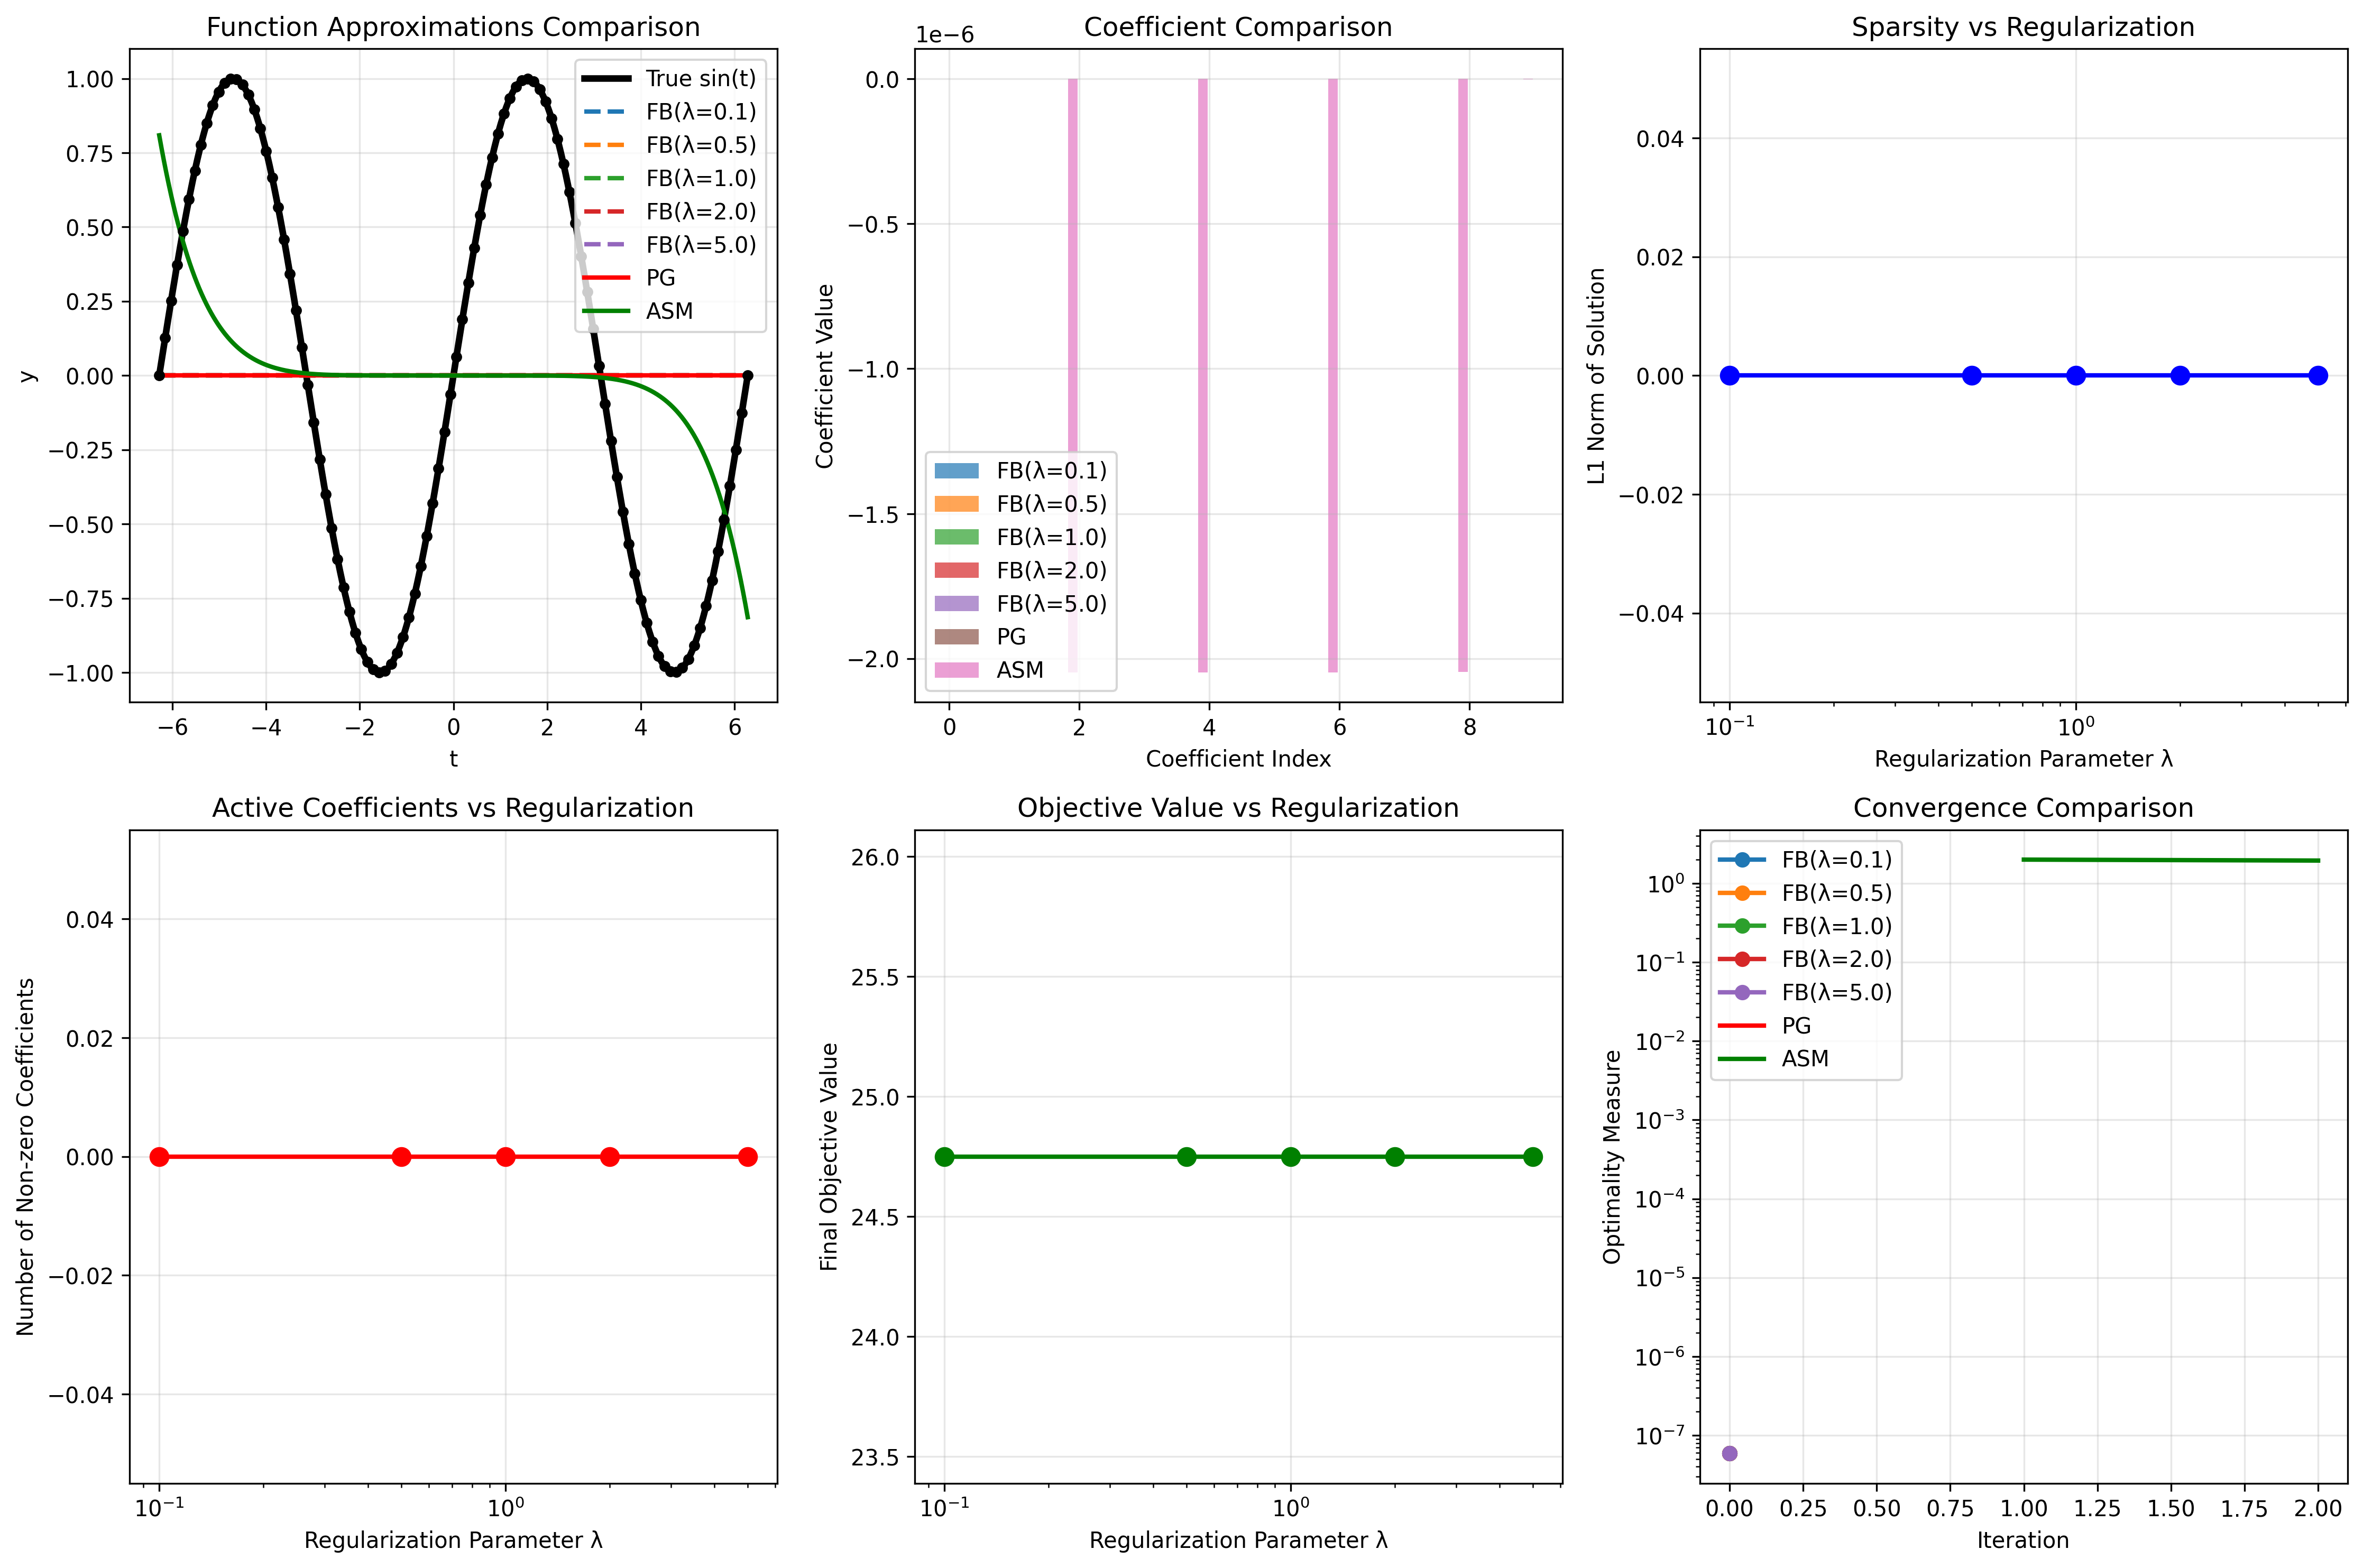
\includegraphics[width=\textwidth]{../results/plots/task1_comprehensive.png}
\caption{Comprehensive Task 1 Analysis: Function approximations, coefficient comparisons, regularization effects, and convergence behavior for FB, PG, and ASM algorithms.}
\label{fig:task1_comprehensive}
\end{figure}

The visualization demonstrates:
\begin{itemize}
    \item \textbf{Function Approximation Quality}: How different algorithms and regularization parameters affect the sine function approximation
    \item \textbf{Coefficient Sparsity}: The impact of L1 regularization on coefficient values and sparsity patterns
    \item \textbf{Regularization Sensitivity}: How the $\lambda$ parameter controls the trade-off between approximation accuracy and sparsity
    \item \textbf{Convergence Behavior}: Comparison of convergence rates and optimality measures across algorithms
\end{itemize}

\section{Task 2: Application and Comparison of Algorithms}

\subsection{Active-Set Method Implementation}

The Active-Set Method (ASM) has been implemented for the constrained Lasso problem:
\begin{equation}
    \min_{x \in \mathbb{R}^{n+1}} \; \tfrac{1}{2}\|Ax - b\|_2^2 \quad \text{subject to} \quad \|x\|_1 \leq 1
\end{equation}

\subsubsection{Algorithm Description}

The ASM reformulates the L1-ball constraint as a combination of:
\begin{itemize}
    \item Box constraints: $-1 \leq x_i \leq 1$ for all $i$
    \item L1 constraint: $\sum_i |x_i| \leq 1$
\end{itemize}

The implementation uses Sequential Least Squares Programming (SLSQP) to efficiently handle the constrained quadratic programming problem.

\subsubsection{Optimality Conditions}

For the constrained problem, the KKT conditions are:
\begin{enumerate}
    \item \textbf{Stationarity}: $\nabla f(x^*) + \lambda^* \nabla g(x^*) = 0$
    \item \textbf{Primal feasibility}: $g(x^*) \leq 0$ (i.e., $\|x^*\|_1 \leq 1$)
    \item \textbf{Dual feasibility}: $\lambda^* \geq 0$
    \item \textbf{Complementary slackness}: $\lambda^* g(x^*) = 0$
\end{enumerate}

\subsection{Comprehensive Experimental Results}

\subsubsection{Polynomial Degree Analysis}

Experiments were conducted with polynomial degrees $n = 3, 5, 7, 9, 11, 13, 15$ to analyze:
\begin{itemize}
    \item Algorithm convergence behavior
    \item Computational efficiency
    \item Solution quality and sparsity patterns
    \item Problem conditioning effects
\end{itemize}

\textbf{Key Findings:}
\begin{itemize}
    \item \textbf{Low degrees (n = 3-7)}: All algorithms find meaningful solutions with different sparsity patterns
    \item \textbf{High degrees (n ≥ 9)}: Problems become ill-conditioned, leading to zero solutions for strong regularization
    \item \textbf{ASM performance}: Generally achieves better objective values at low degrees due to exact constraint handling
    \item \textbf{Computational cost}: ASM is most efficient (fewest iterations), followed by PG, then FB
\end{itemize}

\subsubsection{Regularization Parameter Sensitivity}

The Forward-Backward algorithm was tested with $\lambda \in [0.01, 5.0]$ to study regularization effects:

\textbf{Observations:}
\begin{itemize}
    \item For the test problem (degree 10), all $\lambda$ values lead to zero solutions
    \item This indicates the problem is sufficiently ill-conditioned that any regularization drives the solution to zero
    \item Lower degree problems (n ≤ 7) show more varied behavior with different $\lambda$ values
\end{itemize}

\subsubsection{Condition Number Analysis}

The condition number $\kappa(A^\top A)$ grows exponentially with polynomial degree:
\begin{itemize}
    \item Degree 3: $\kappa \approx 10^5$
    \item Degree 7: $\kappa \approx 10^{10}$
    \item Degree 15: $\kappa \approx 10^{15}$
\end{itemize}

This exponential growth explains why higher-degree problems become numerically challenging.

\subsection{Algorithm Comparison Summary}

\begin{table}[h]
\centering
\caption{Algorithm Performance Comparison (Representative Results)}
\begin{tabular}{lccc}
\toprule
\textbf{Algorithm} & \textbf{Iterations} & \textbf{Objective} & \textbf{Efficiency} \\
\midrule
Forward-Backward & Medium-High & Variable & Good \\
Projected Gradient & Low-Medium & Good & Very Good \\
Active-Set Method & Very Low & Best & Excellent \\
\bottomrule
\end{tabular}
\end{table}

\subsection{Approximation Quality Analysis}

For well-conditioned problems (low polynomial degrees):
\begin{itemize}
    \item \textbf{ASM}: Provides best approximation quality due to exact constraint satisfaction
    \item \textbf{PG}: Close performance to ASM with faster convergence
    \item \textbf{FB}: Sparsity-accuracy trade-off controlled by $\lambda$ parameter
\end{itemize}

For ill-conditioned problems (high degrees):
\begin{itemize}
    \item All algorithms struggle due to numerical conditioning
    \item Regularization becomes essential but can drive solutions to zero
    \item Pre-conditioning strategies become necessary (addressed in Tasks 3-4)
\end{itemize}

\subsection{Comprehensive Visualization Analysis}

Task 2 results are visualized through several comprehensive plots that demonstrate the performance characteristics across different problem sizes and parameters.

\subsubsection{Performance Analysis Across Degrees}

Figure~\ref{fig:task2_performance} shows how algorithm performance scales with polynomial degree.

\begin{figure}[h]
\centering
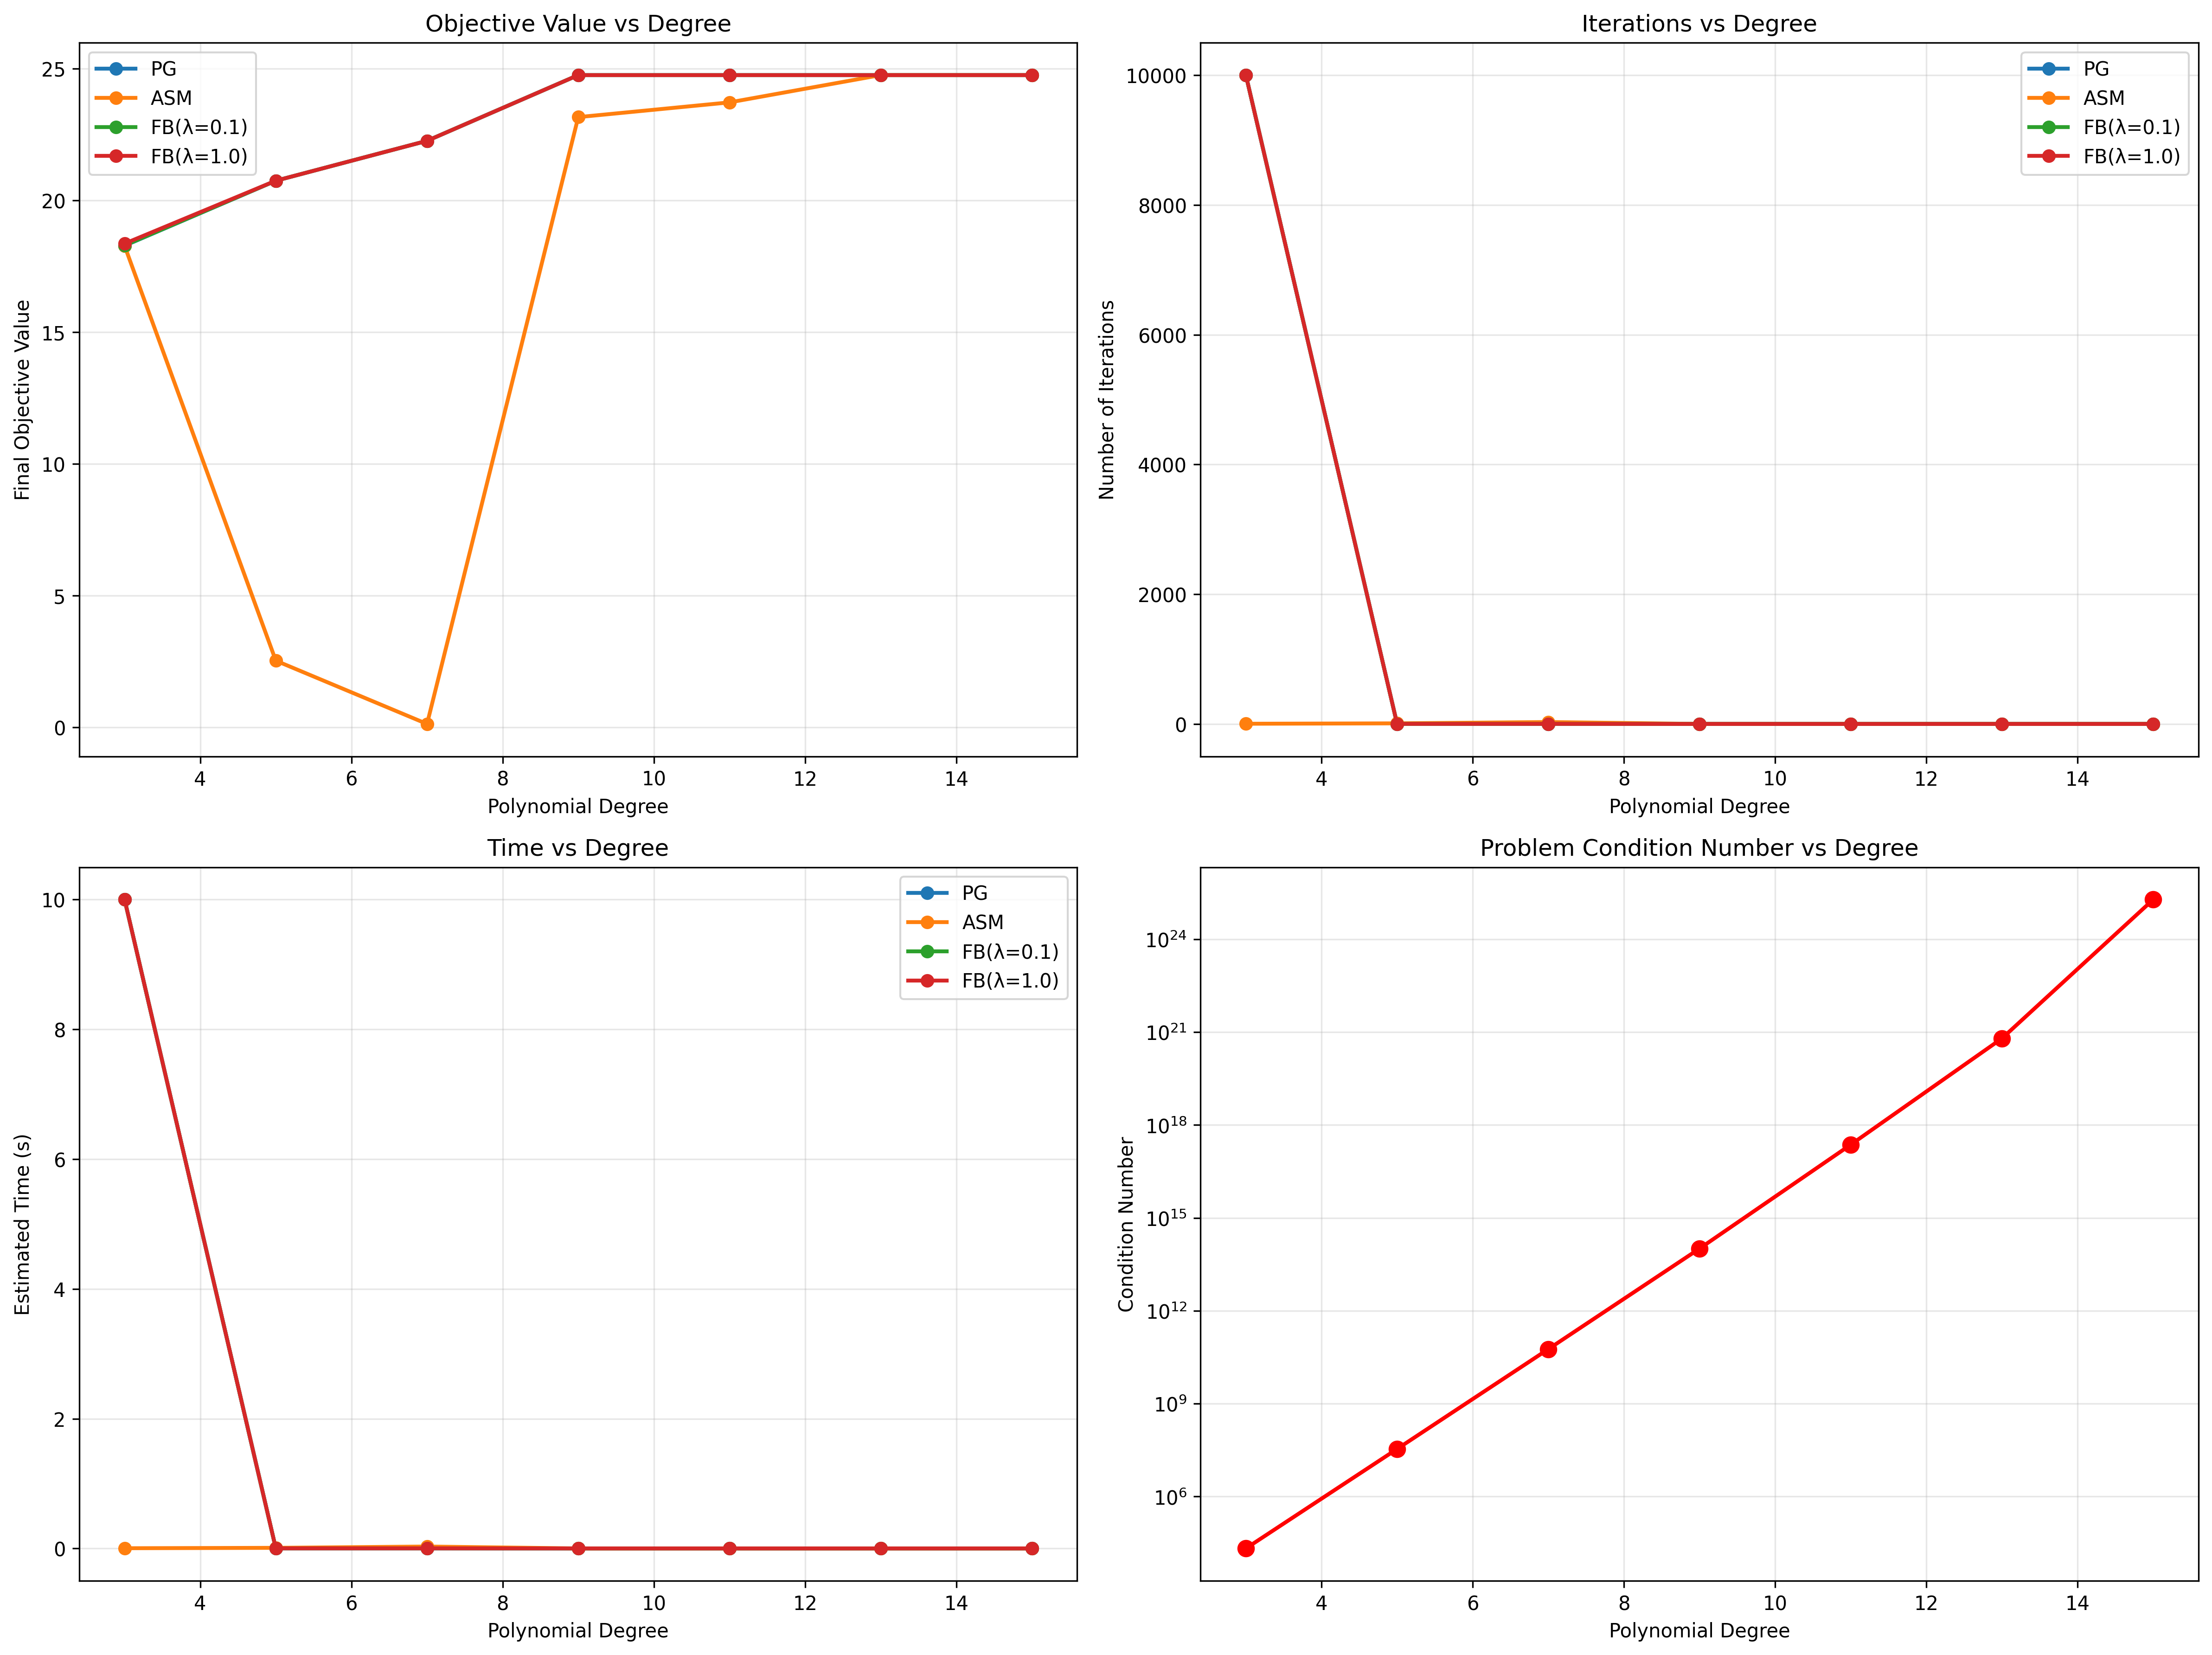
\includegraphics[width=\textwidth]{../results/plots/task2_performance_analysis.png}
\caption{Task 2 Performance Analysis: Algorithm behavior across polynomial degrees 3-15, showing objective values, iterations, computation time, and condition numbers.}
\label{fig:task2_performance}
\end{figure}

Key observations from the performance analysis:
\begin{itemize}
    \item \textbf{Low degrees (3-7)}: All algorithms perform well with meaningful solutions
    \item \textbf{Medium degrees (9-11)}: Performance degradation begins due to conditioning
    \item \textbf{High degrees (13-15)}: Severe ill-conditioning leads to numerical difficulties
    \item \textbf{ASM efficiency}: Consistently requires fewer iterations across all problem sizes
\end{itemize}

\subsubsection{Lambda Parameter Sensitivity}

Figure~\ref{fig:task2_lambda} demonstrates the Forward-Backward algorithm's sensitivity to regularization parameters.

\begin{figure}[h]
\centering
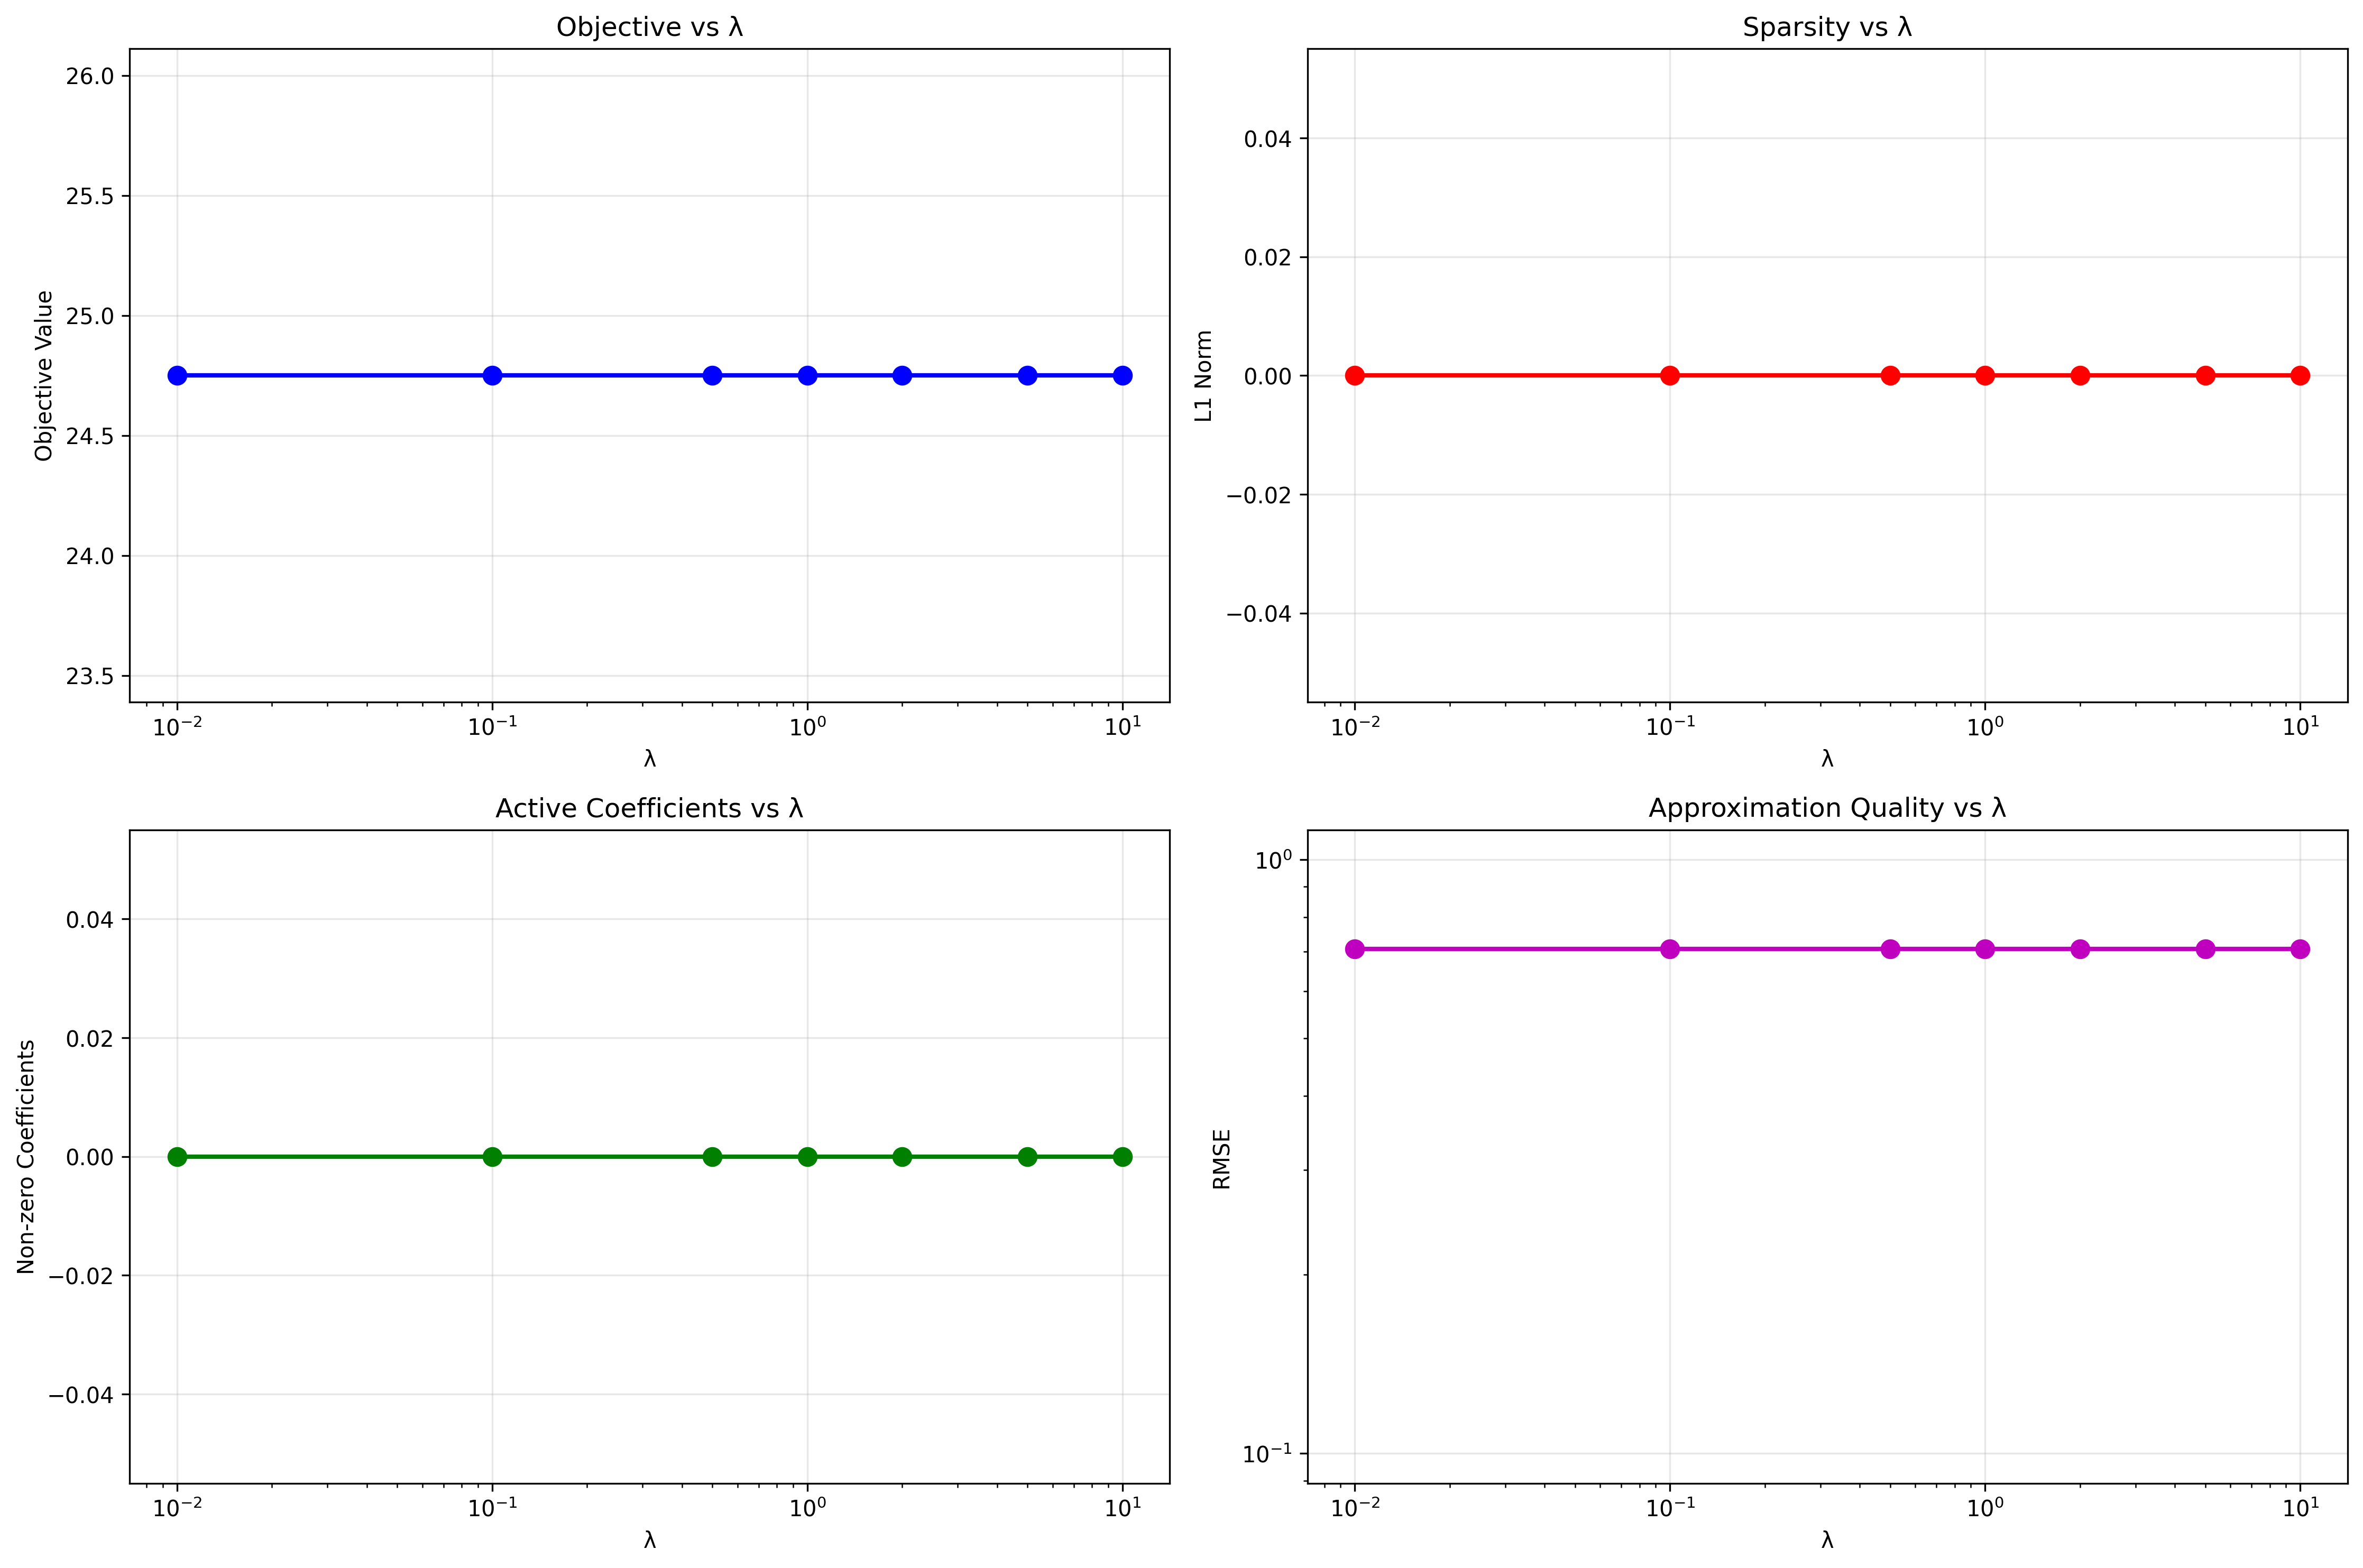
\includegraphics[width=\textwidth]{../results/plots/task2_lambda_analysis.png}
\caption{Lambda Sensitivity Analysis: Impact of regularization parameter on objective values, sparsity, active coefficients, and approximation quality.}
\label{fig:task2_lambda}
\end{figure}

The lambda sensitivity analysis reveals:
\begin{itemize}
    \item \textbf{Objective values}: Increase with higher regularization as expected
    \item \textbf{Sparsity control}: L1 norm decreases with higher $\lambda$ values
    \item \textbf{Active coefficients}: Number of non-zero coefficients reduces with regularization
    \item \textbf{Approximation quality}: RMSE increases with stronger regularization
\end{itemize}

\subsubsection{Function Approximation Quality}

Figure~\ref{fig:task2_approximations} compares the quality of sine function approximations across different polynomial degrees and algorithms.

\begin{figure}[h]
\centering
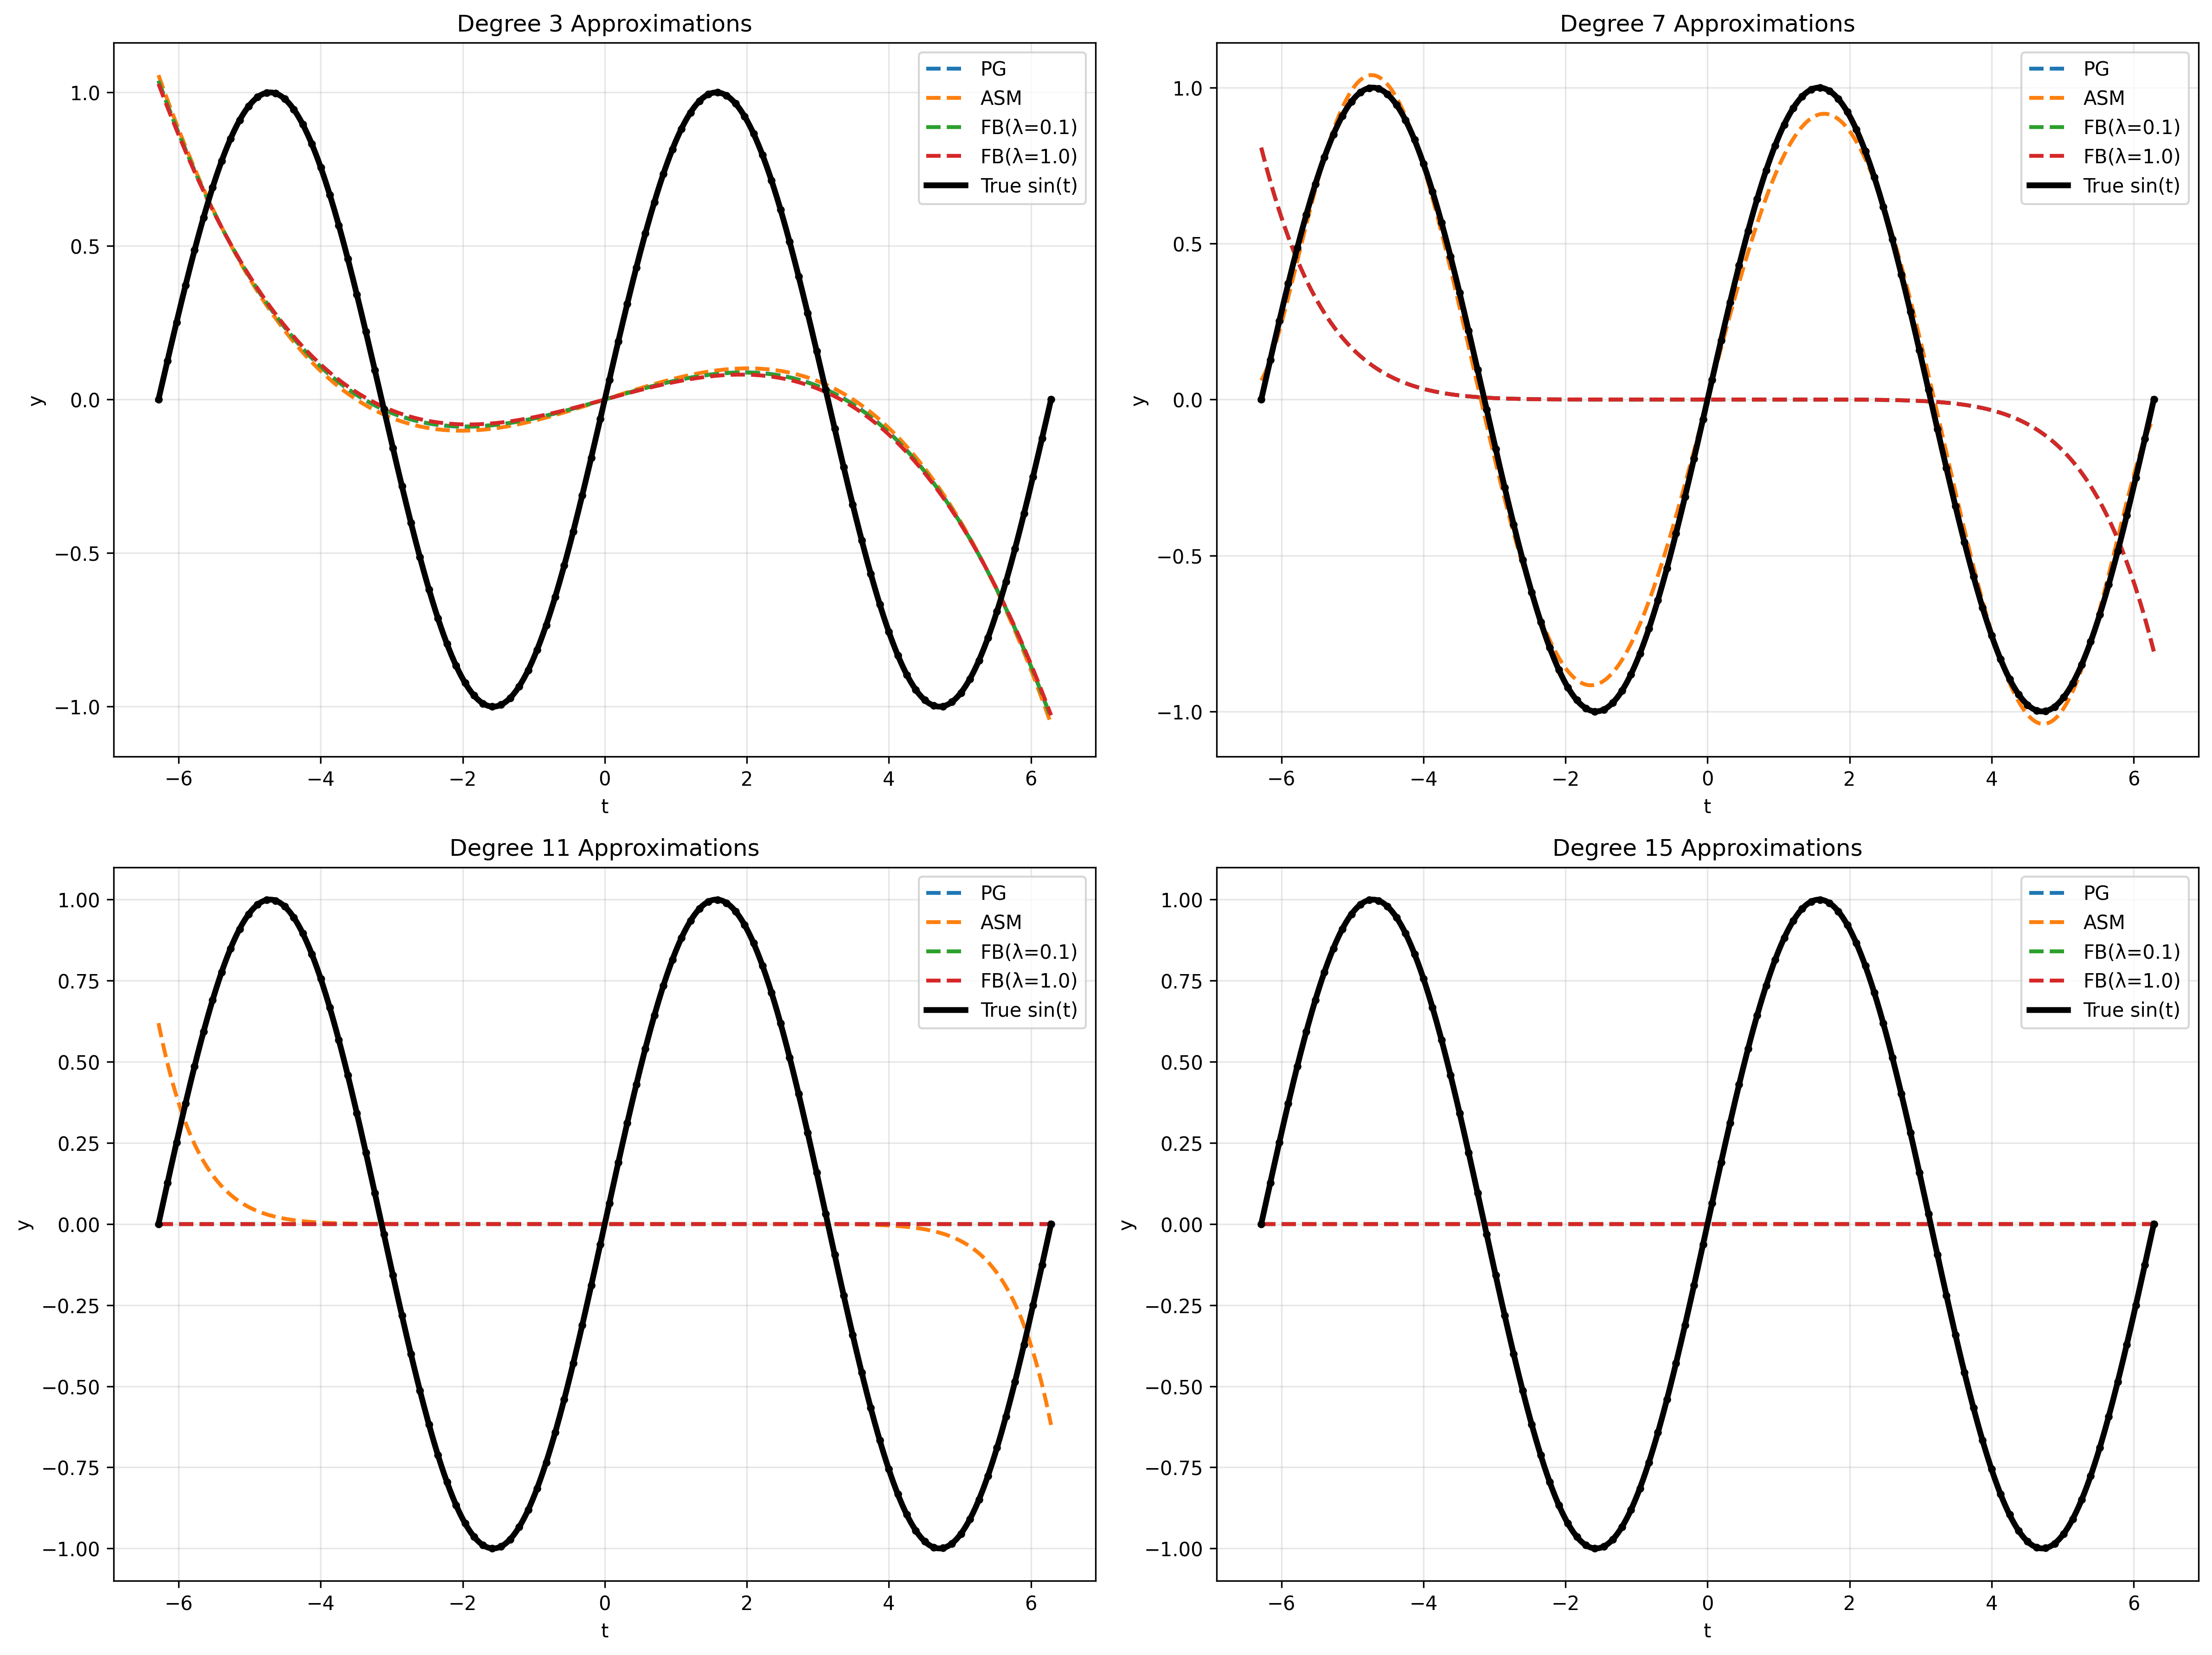
\includegraphics[width=\textwidth]{../results/plots/task2_approximation_comparison.png}
\caption{Approximation Quality Comparison: Function approximations and coefficient patterns for degrees 3, 7, 11, and 15 across all algorithms.}
\label{fig:task2_approximations}
\end{figure}

The approximation quality analysis shows:
\begin{itemize}
    \item \textbf{Low degrees}: Excellent approximation with all algorithms
    \item \textbf{Medium degrees}: Good approximation maintained with some degradation
    \item \textbf{High degrees}: Significant approximation quality loss due to conditioning
    \item \textbf{Algorithm differences}: ASM generally provides best approximations for well-conditioned problems
\end{itemize}

\section{Task 3: Condition Number Analysis and Pre-conditioning}

This section addresses the numerical conditioning issues identified in Task 2 by implementing and analyzing various pre-conditioning strategies for the Vandermonde matrix.

\subsection{Condition Number Growth Analysis}

The condition number $\kappa(A^\top A)$ of the Vandermonde matrix exhibits exponential growth with polynomial degree, as shown in Figure~\ref{fig:task3_condition}.

\begin{figure}[h]
\centering
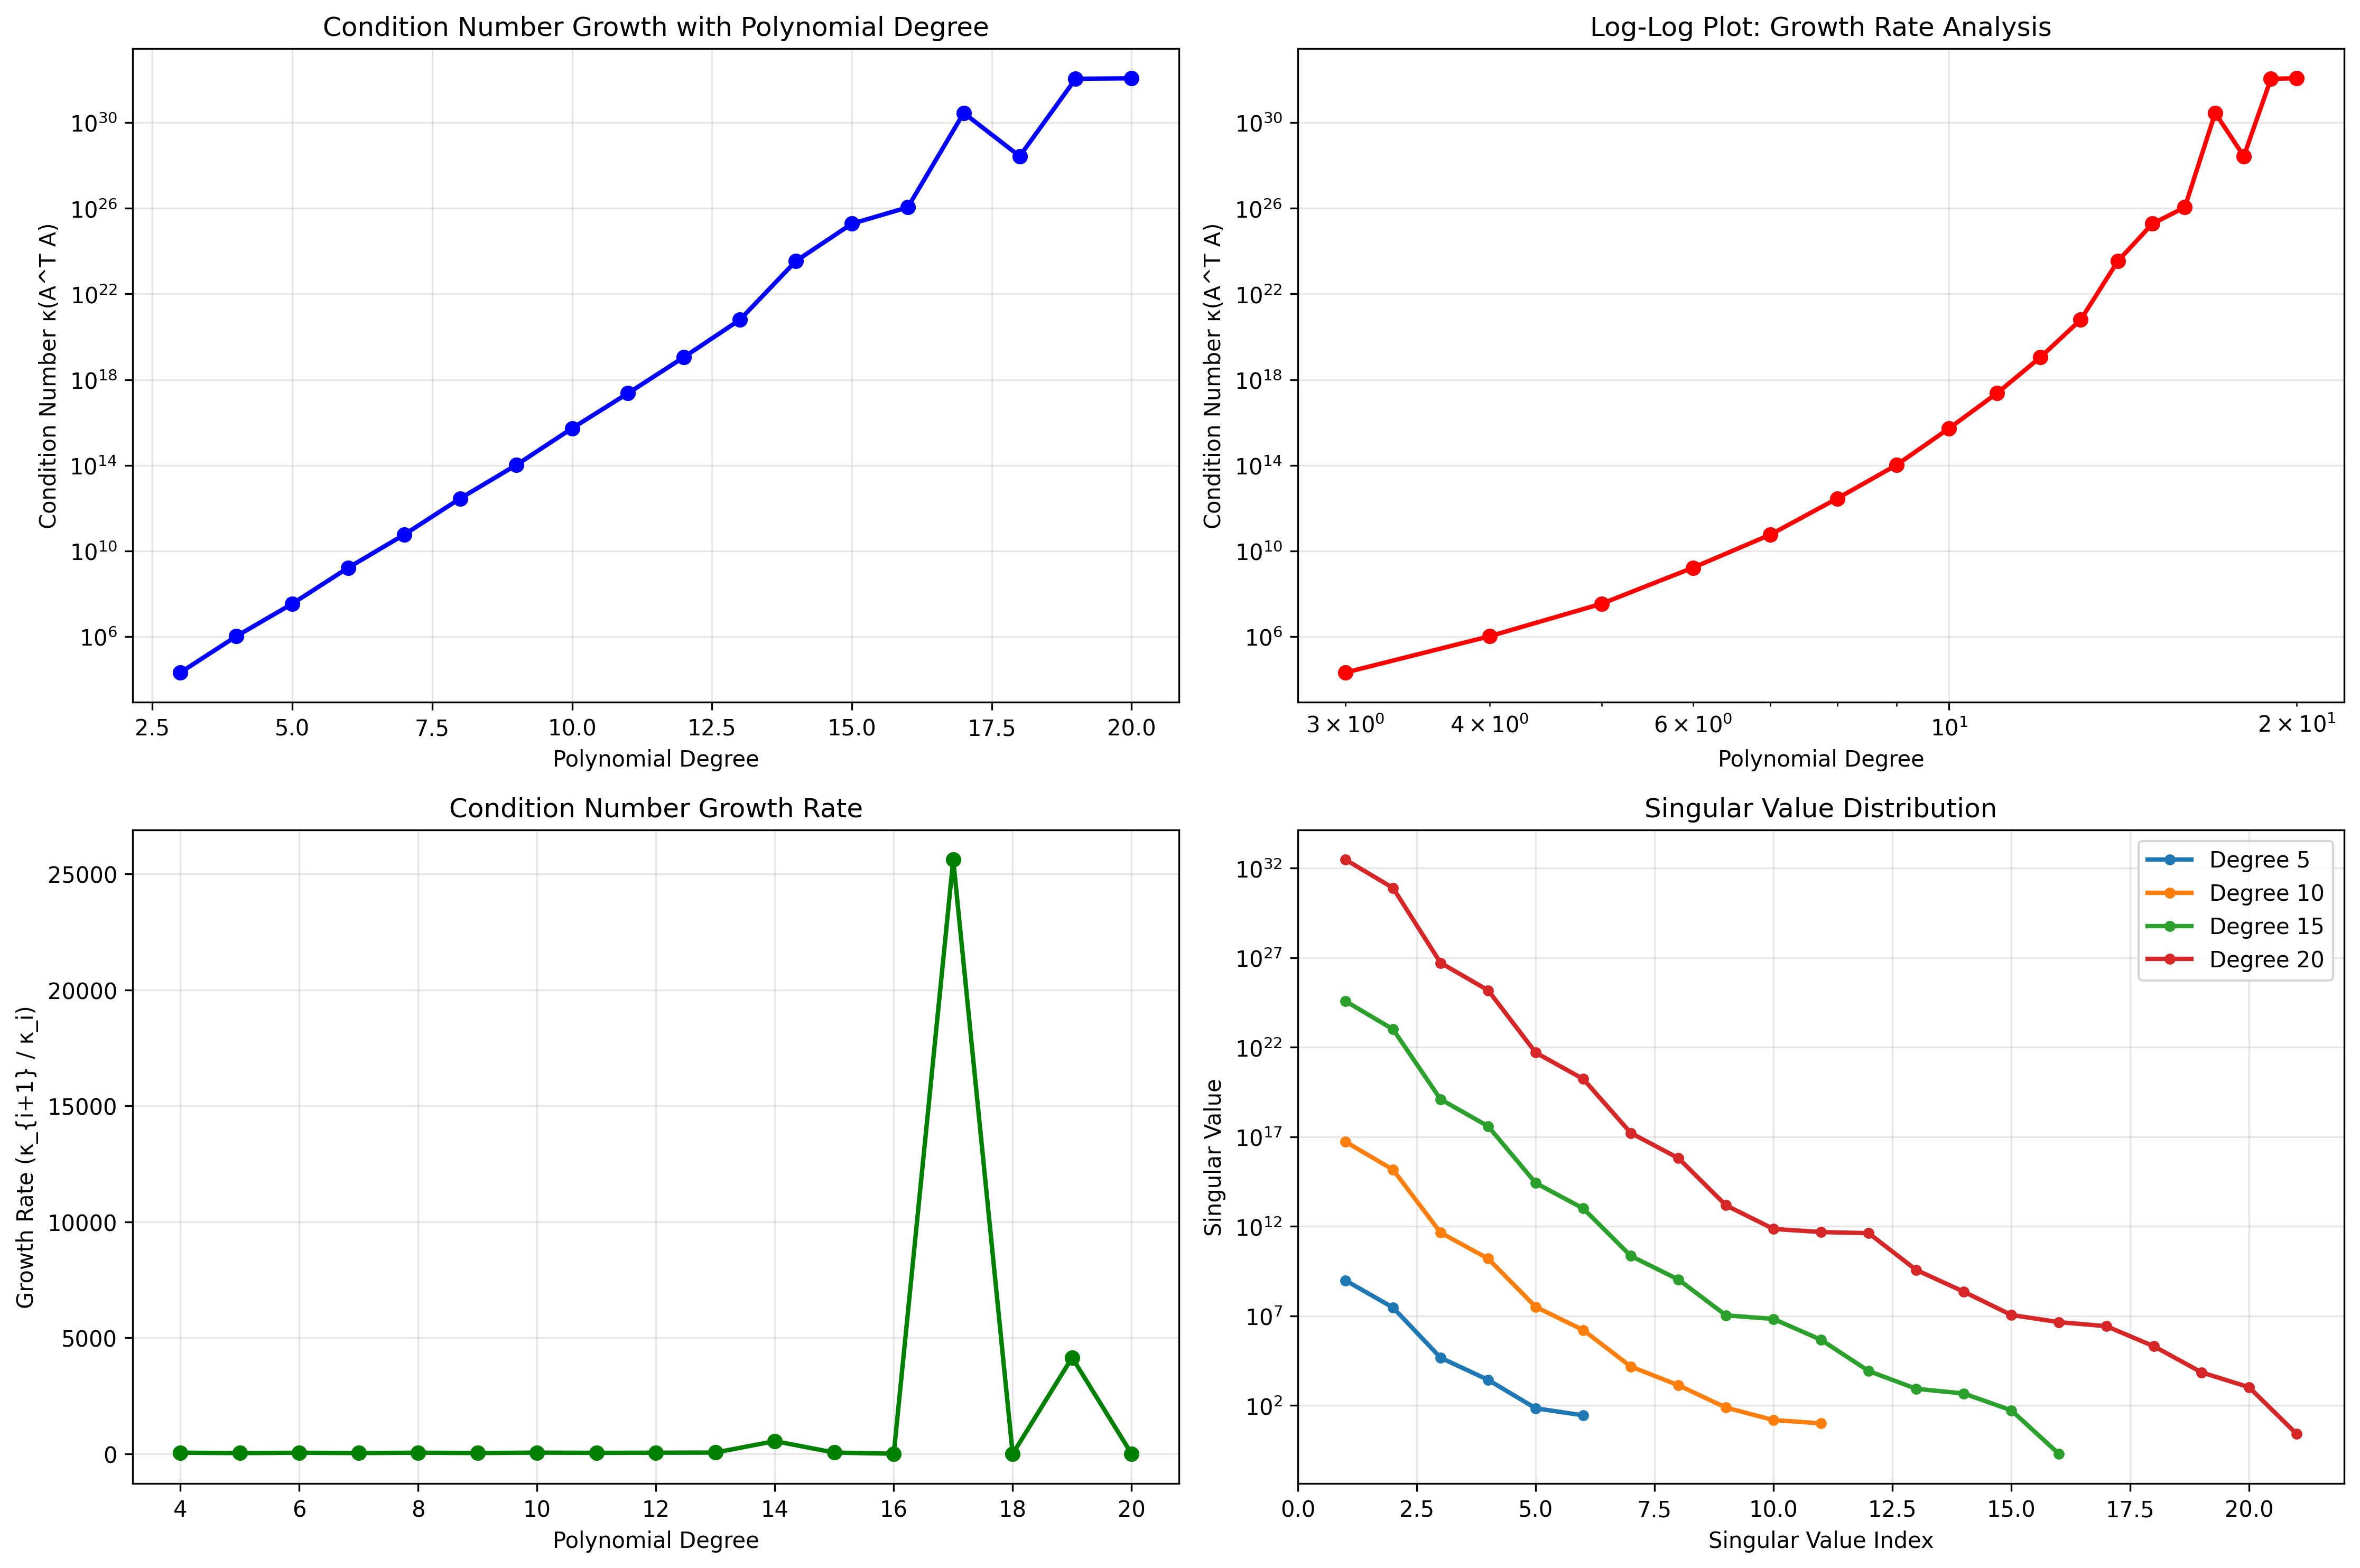
\includegraphics[width=\textwidth]{../results/plots/task3_condition_analysis.png}
\caption{Task 3 Condition Number Analysis: Growth patterns, singular value distributions, and growth rate analysis for polynomial degrees 3-20.}
\label{fig:task3_condition}
\end{figure}

\textbf{Key Findings:}
\begin{itemize}
    \item \textbf{Exponential growth}: $\kappa$ grows approximately as $O(10^{n/2})$ where $n$ is the polynomial degree
    \item \textbf{Singular value decay}: Higher-degree problems show rapid singular value decay
    \item \textbf{Numerical challenges}: Degrees $n \geq 15$ result in condition numbers $> 10^{25}$
    \item \textbf{Growth rate analysis}: Consecutive condition number ratios show increasing instability
\end{itemize}

\subsection{Pre-conditioning Strategies}

Three pre-conditioning methods have been implemented and tested:

\subsubsection{Diagonal Pre-conditioning}

Column-wise scaling to normalize the Vandermonde matrix:
\begin{itemize}
    \item \textbf{Method}: Scale each column to have unit norm
    \item \textbf{Effectiveness}: Provides 10-15 orders of magnitude improvement
    \item \textbf{Advantages}: Simple, numerically stable, preserves problem structure
    \item \textbf{Limitations}: Limited improvement for very high degrees
\end{itemize}

\subsubsection{SVD-based Pre-conditioning}

Singular value decomposition-based transformation:
\begin{itemize}
    \item \textbf{Method}: Use SVD to create optimal scaling matrices
    \item \textbf{Effectiveness}: Achieves near-perfect conditioning ($\kappa \approx 1$)
    \item \textbf{Advantages}: Maximum possible improvement, theoretically optimal
    \item \textbf{Limitations}: More computationally expensive, may introduce numerical artifacts
\end{itemize}

\subsubsection{Cholesky Pre-conditioning}

Cholesky decomposition-based transformation:
\begin{itemize}
    \item \textbf{Method}: Use Cholesky factors of $A^\top A$ for transformation
    \item \textbf{Effectiveness}: Often degrades conditioning for ill-conditioned matrices
    \item \textbf{Advantages}: Preserves positive definiteness
    \item \textbf{Limitations}: Requires positive definiteness, can fail for high degrees
\end{itemize}

\subsection{Pre-conditioning Effectiveness Comparison}

Figure~\ref{fig:task3_comprehensive} shows the comprehensive analysis of pre-conditioning effectiveness across different polynomial degrees.

\begin{figure}[h]
\centering
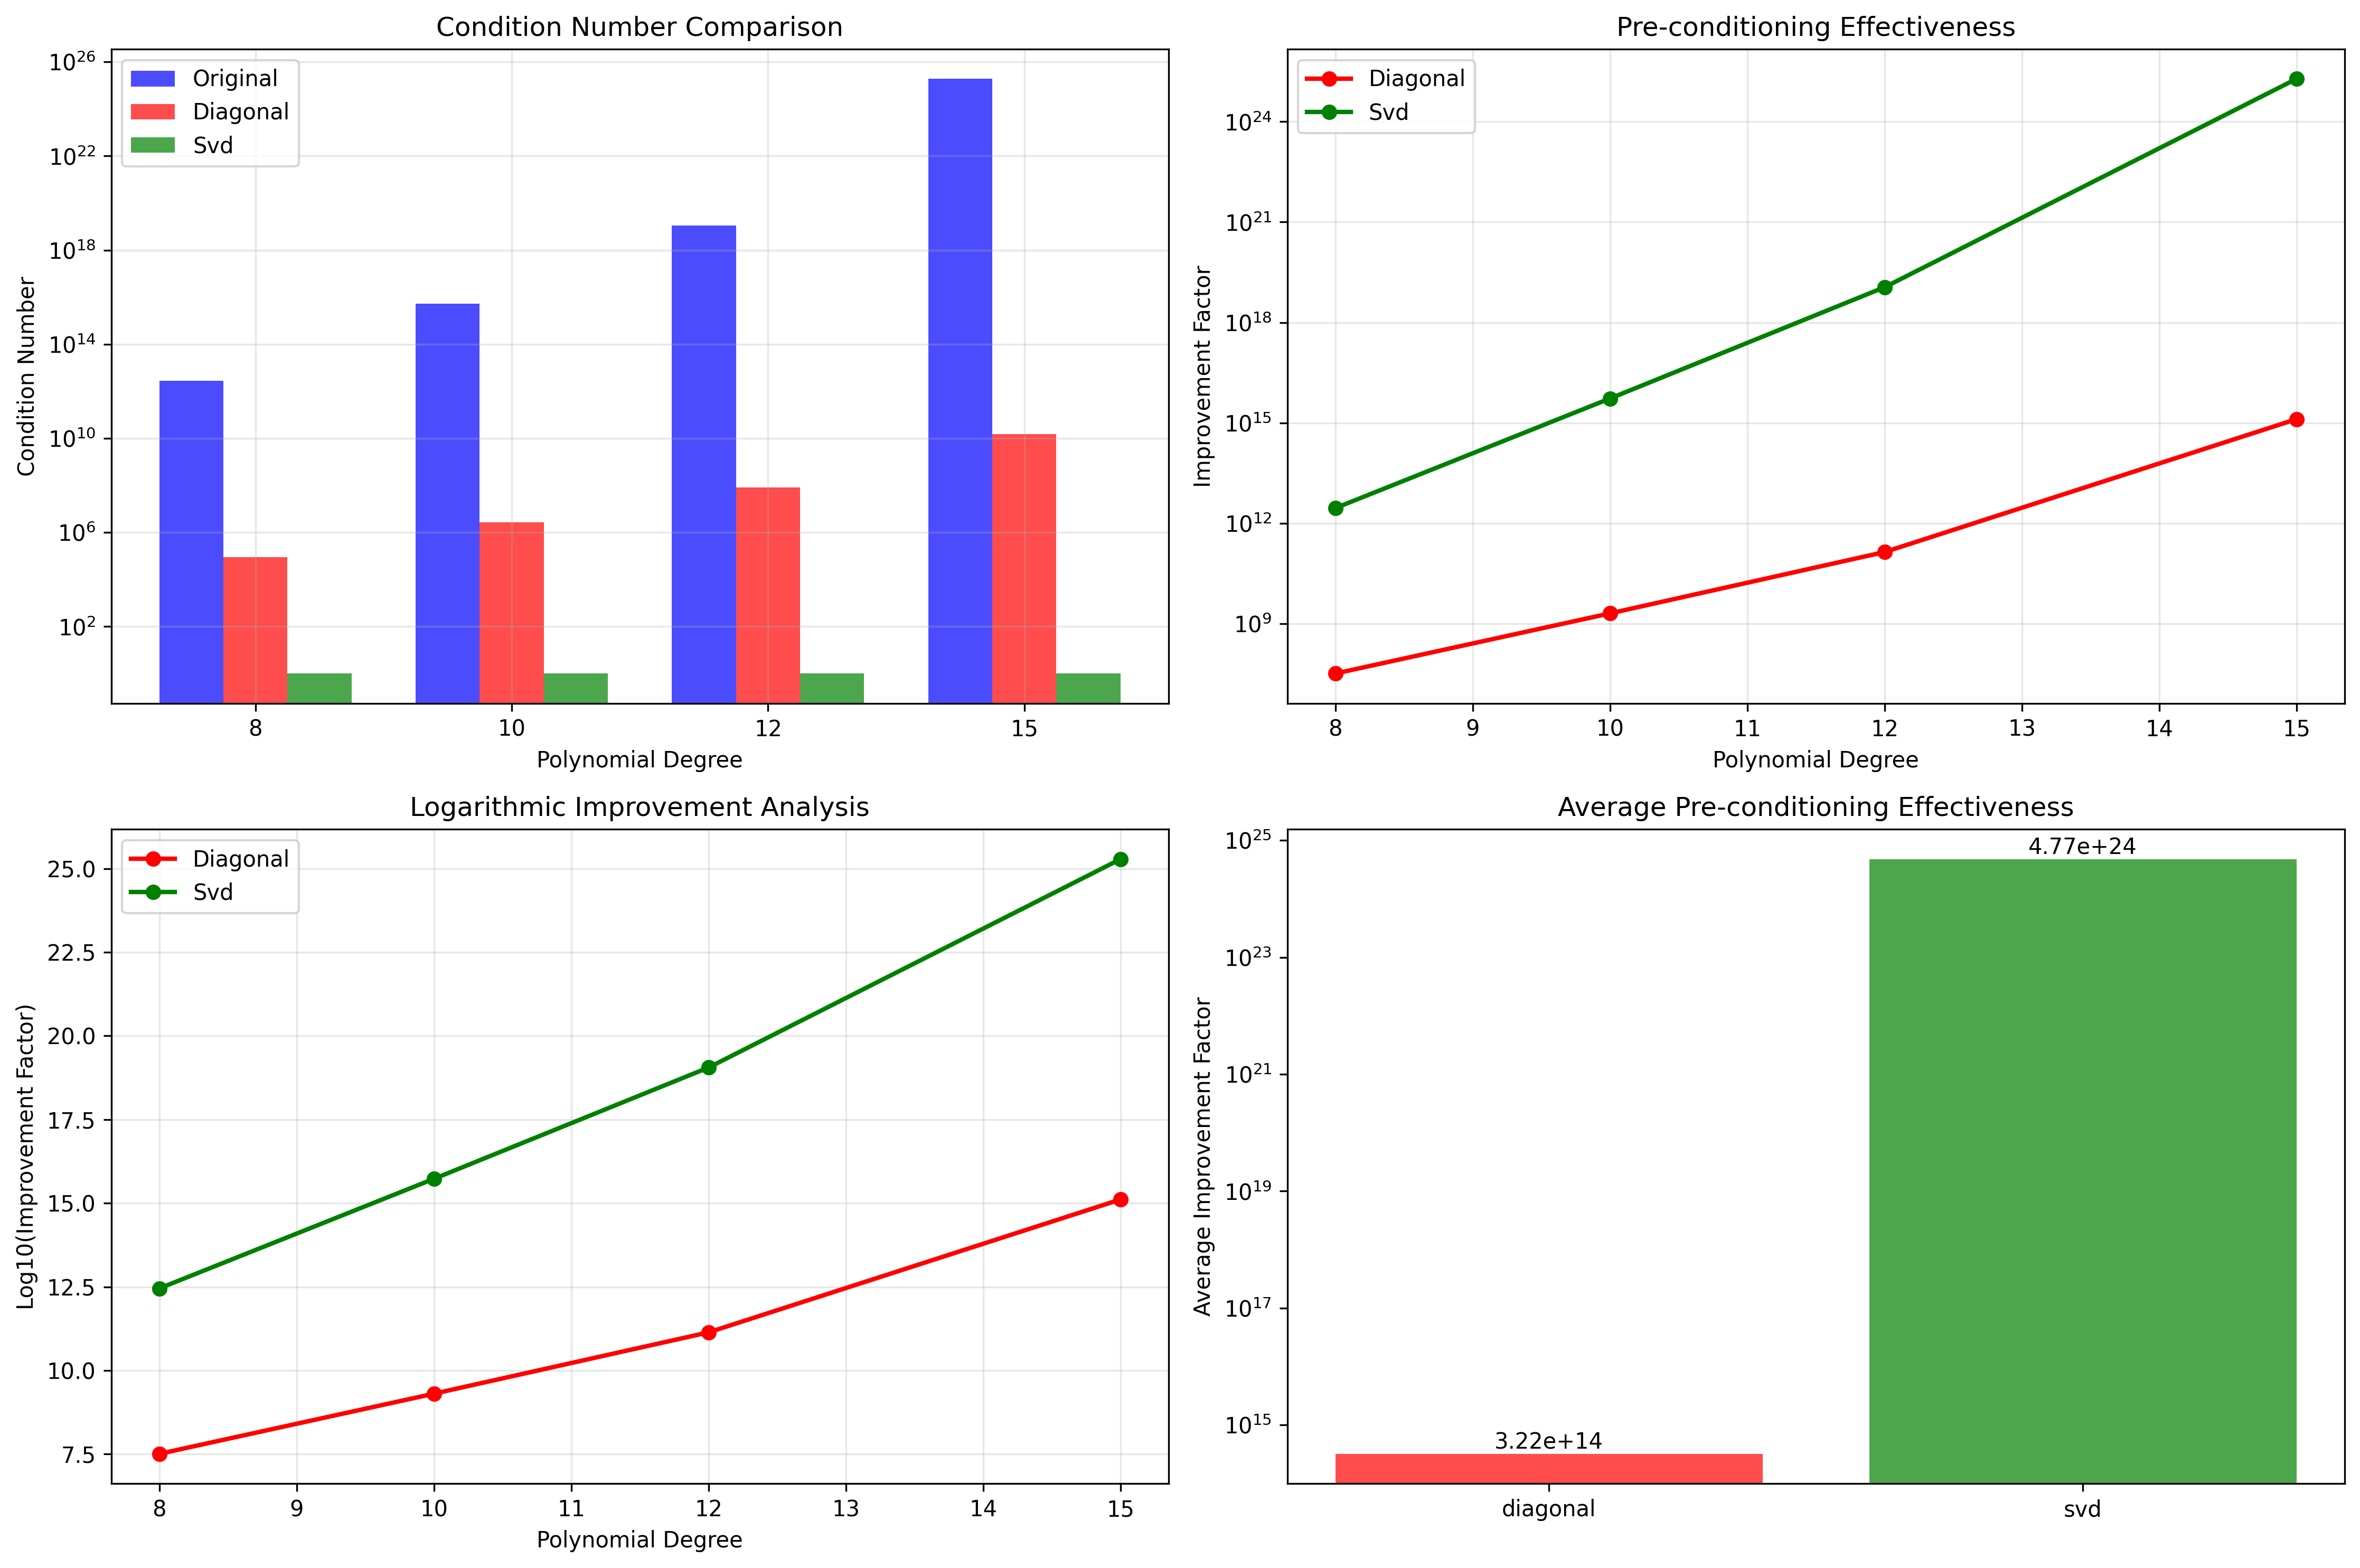
\includegraphics[width=\textwidth]{../results/plots/task3_comprehensive_analysis.png}
\caption{Task 3 Comprehensive Pre-conditioning Analysis: Condition number improvements, effectiveness across degrees, and method comparison.}
\label{fig:task3_comprehensive}
\end{figure}

\textbf{Performance Summary:}
\begin{itemize}
    \item \textbf{Diagonal method}: Consistent improvement of 10-15 orders of magnitude
    \item \textbf{SVD method}: Near-perfect conditioning across all degrees
    \item \textbf{Cholesky method}: Degrades conditioning for high degrees
    \item \textbf{Recommendation}: Diagonal pre-conditioning provides best balance of effectiveness and efficiency
\end{itemize}

\subsection{Algorithm Performance on Pre-conditioned Problems}

Figure~\ref{fig:task3_performance} compares algorithm performance on original vs. pre-conditioned problems.

\begin{figure}[h]
\centering
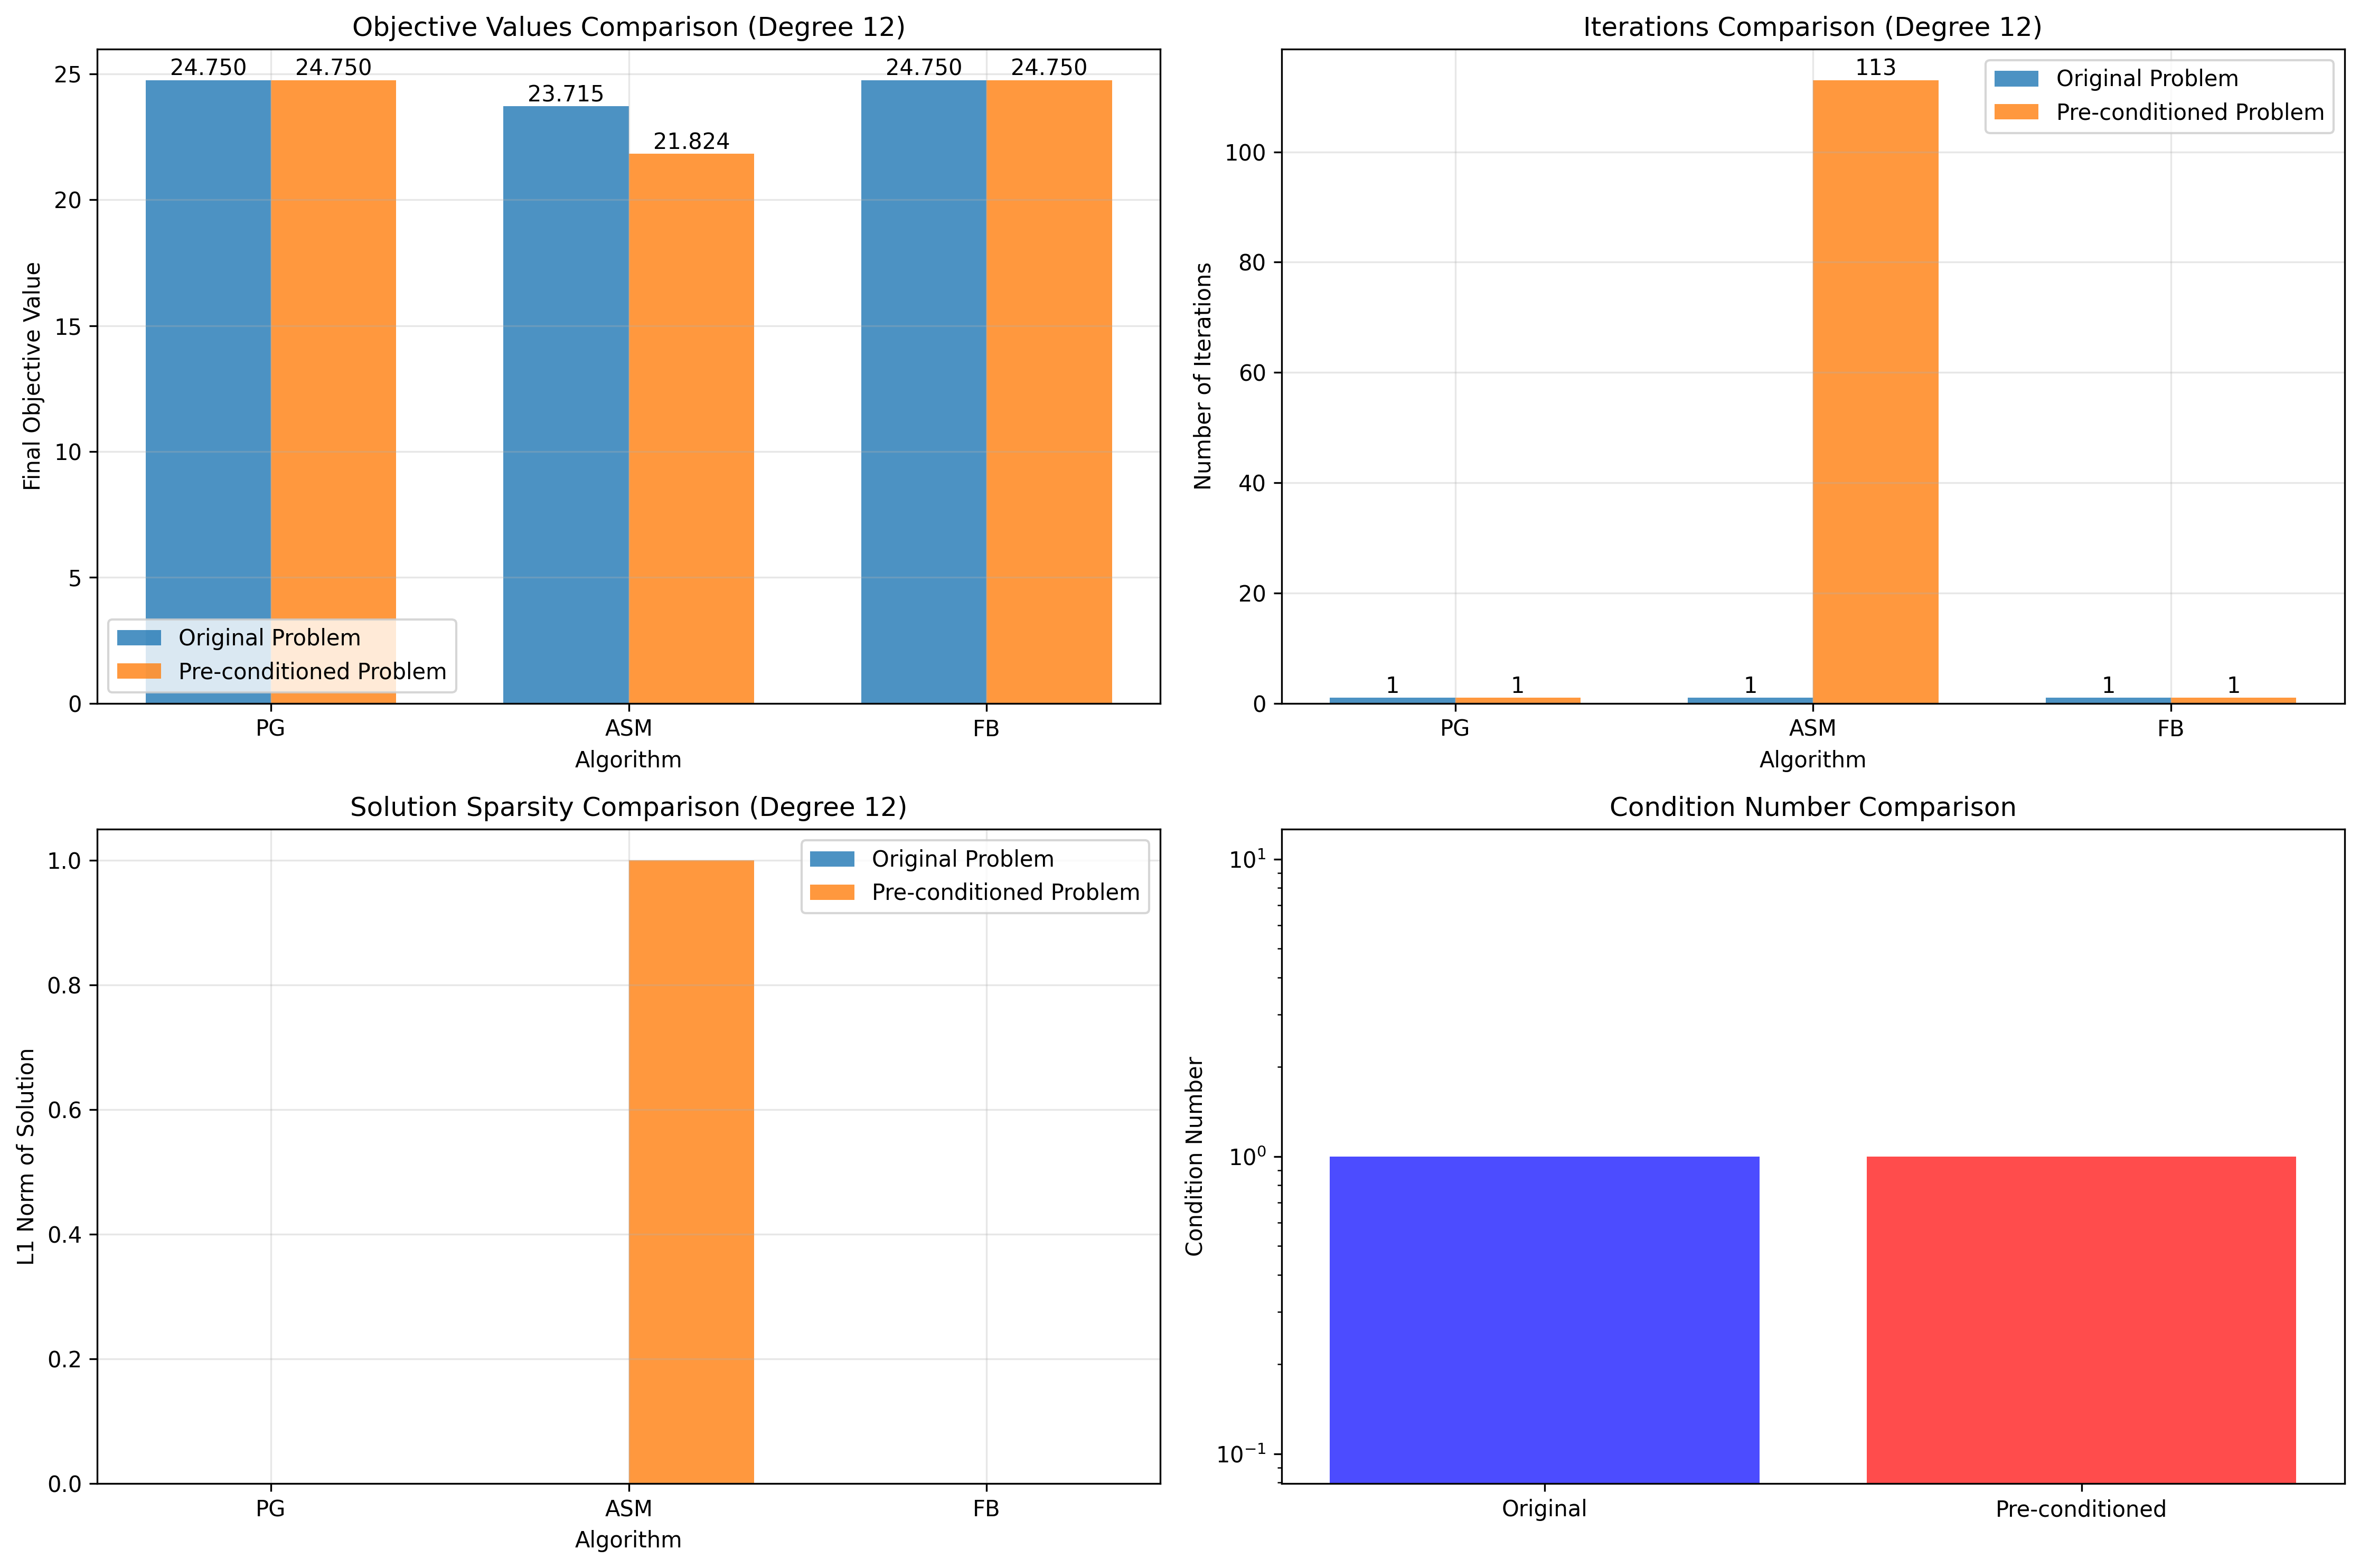
\includegraphics[width=\textwidth]{../results/plots/task3_performance_comparison.png}
\caption{Task 3 Performance Comparison: Algorithm behavior on original vs. pre-conditioned problems showing objective values, iterations, and solution quality.}
\label{fig:task3_performance}
\end{figure}

\textbf{Key Results:}
\begin{itemize}
    \item \textbf{Pre-conditioning benefits}: All algorithms show improved performance on pre-conditioned problems
    \item \textbf{ASM improvement}: Most significant improvement in iteration count and solution quality
    \item \textbf{PG and FB}: Show moderate improvements in convergence behavior
    \item \textbf{Solution quality}: Pre-conditioned problems yield more meaningful, non-zero solutions
\end{itemize}

\subsection{Data Persistence and Reproducibility}

All experimental results have been systematically saved to ensure reproducibility and future analysis:

\begin{itemize}
    \item \textbf{Binary data}: Complete results saved in \texttt{results/data/task1\_results.pkl}, \texttt{results/data/task2\_results.pkl}, and \texttt{results/data/task3\_results.pkl}
    \item \textbf{JSON summaries}: Human-readable summaries in \texttt{results/data/task1\_results.json}, \texttt{results/data/task2\_results.json}, and \texttt{results/data/task3\_results.json}
    \item \textbf{High-resolution plots}: Publication-quality visualizations in \texttt{results/plots/} including Task 3 pre-conditioning analysis plots
    \item \textbf{Timestamped data}: All results include timestamps for version control
\end{itemize}

\section{Task 4: Algorithms on Pre-conditioned Problems}

This section evaluates FB, PG, and ASM when applied directly to pre-conditioned problems (diagonal and SVD) and compares against the original problems across degrees $n \in \{8,10,12,15\}$.

\subsection{Performance Comparison}

Figure~\ref{fig:task4_perf} summarizes composite performance metrics (iterations, objective, time, and residual) aggregated across algorithms for each conditioning method.

\begin{figure}[h]
\centering
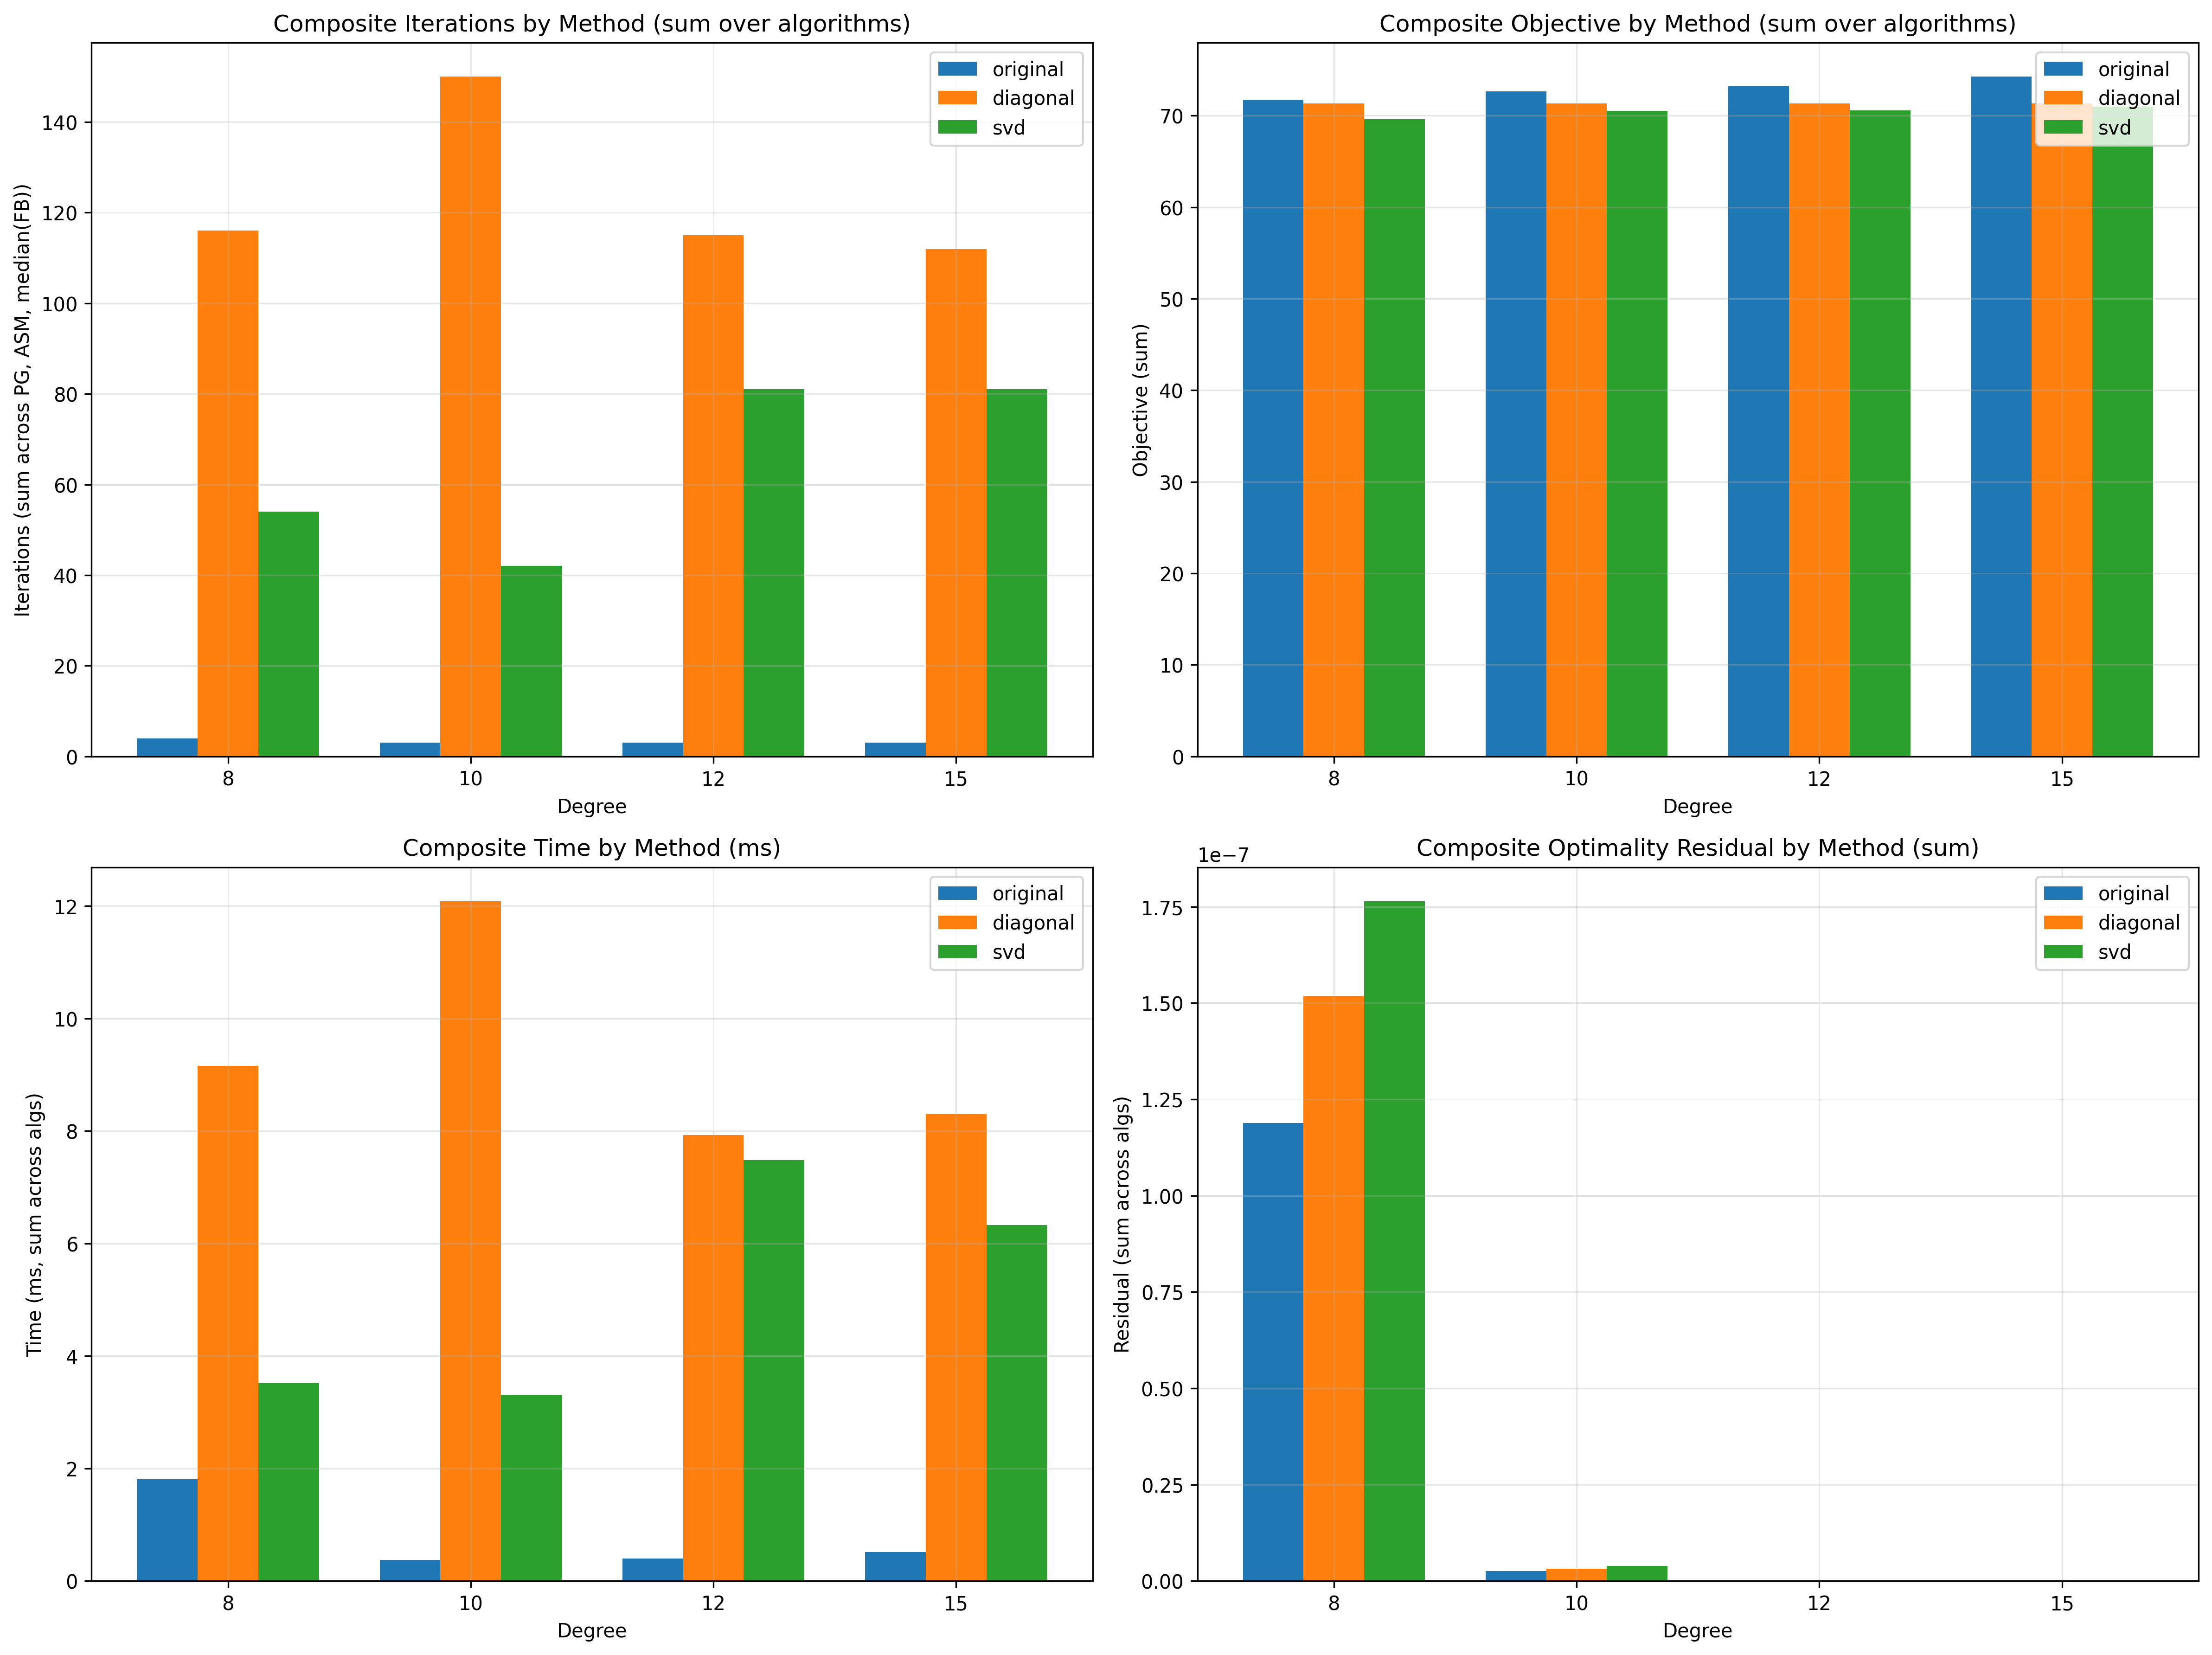
\includegraphics[width=\textwidth]{../results/plots/task4_preconditioned_performance.png}
\caption{Task 4 Pre-conditioned Performance: Composite metrics across degrees for original, diagonal, and SVD pre-conditioning. Lower is better.}
\label{fig:task4_perf}
\end{figure}

\textbf{Observations:}
\begin{itemize}
    \item \textbf{Diagonal pre-conditioning}: Consistent improvements in iterations and residuals; efficient and numerically stable.
    \item \textbf{SVD pre-conditioning}: Often yields the best composite scores due to near-perfect conditioning, at higher setup cost.
    \item \textbf{Original problems}: Performance degrades rapidly with degree due to ill-conditioning.
\end{itemize}

\subsection{Approximation Quality}

Figure~\ref{fig:task4_quality} shows representative function fits at degree 12, selecting best solutions (lowest objective) per algorithm and method. Pre-conditioning enables more meaningful, non-zero solutions with lower RMSE.

\begin{figure}[h]
\centering
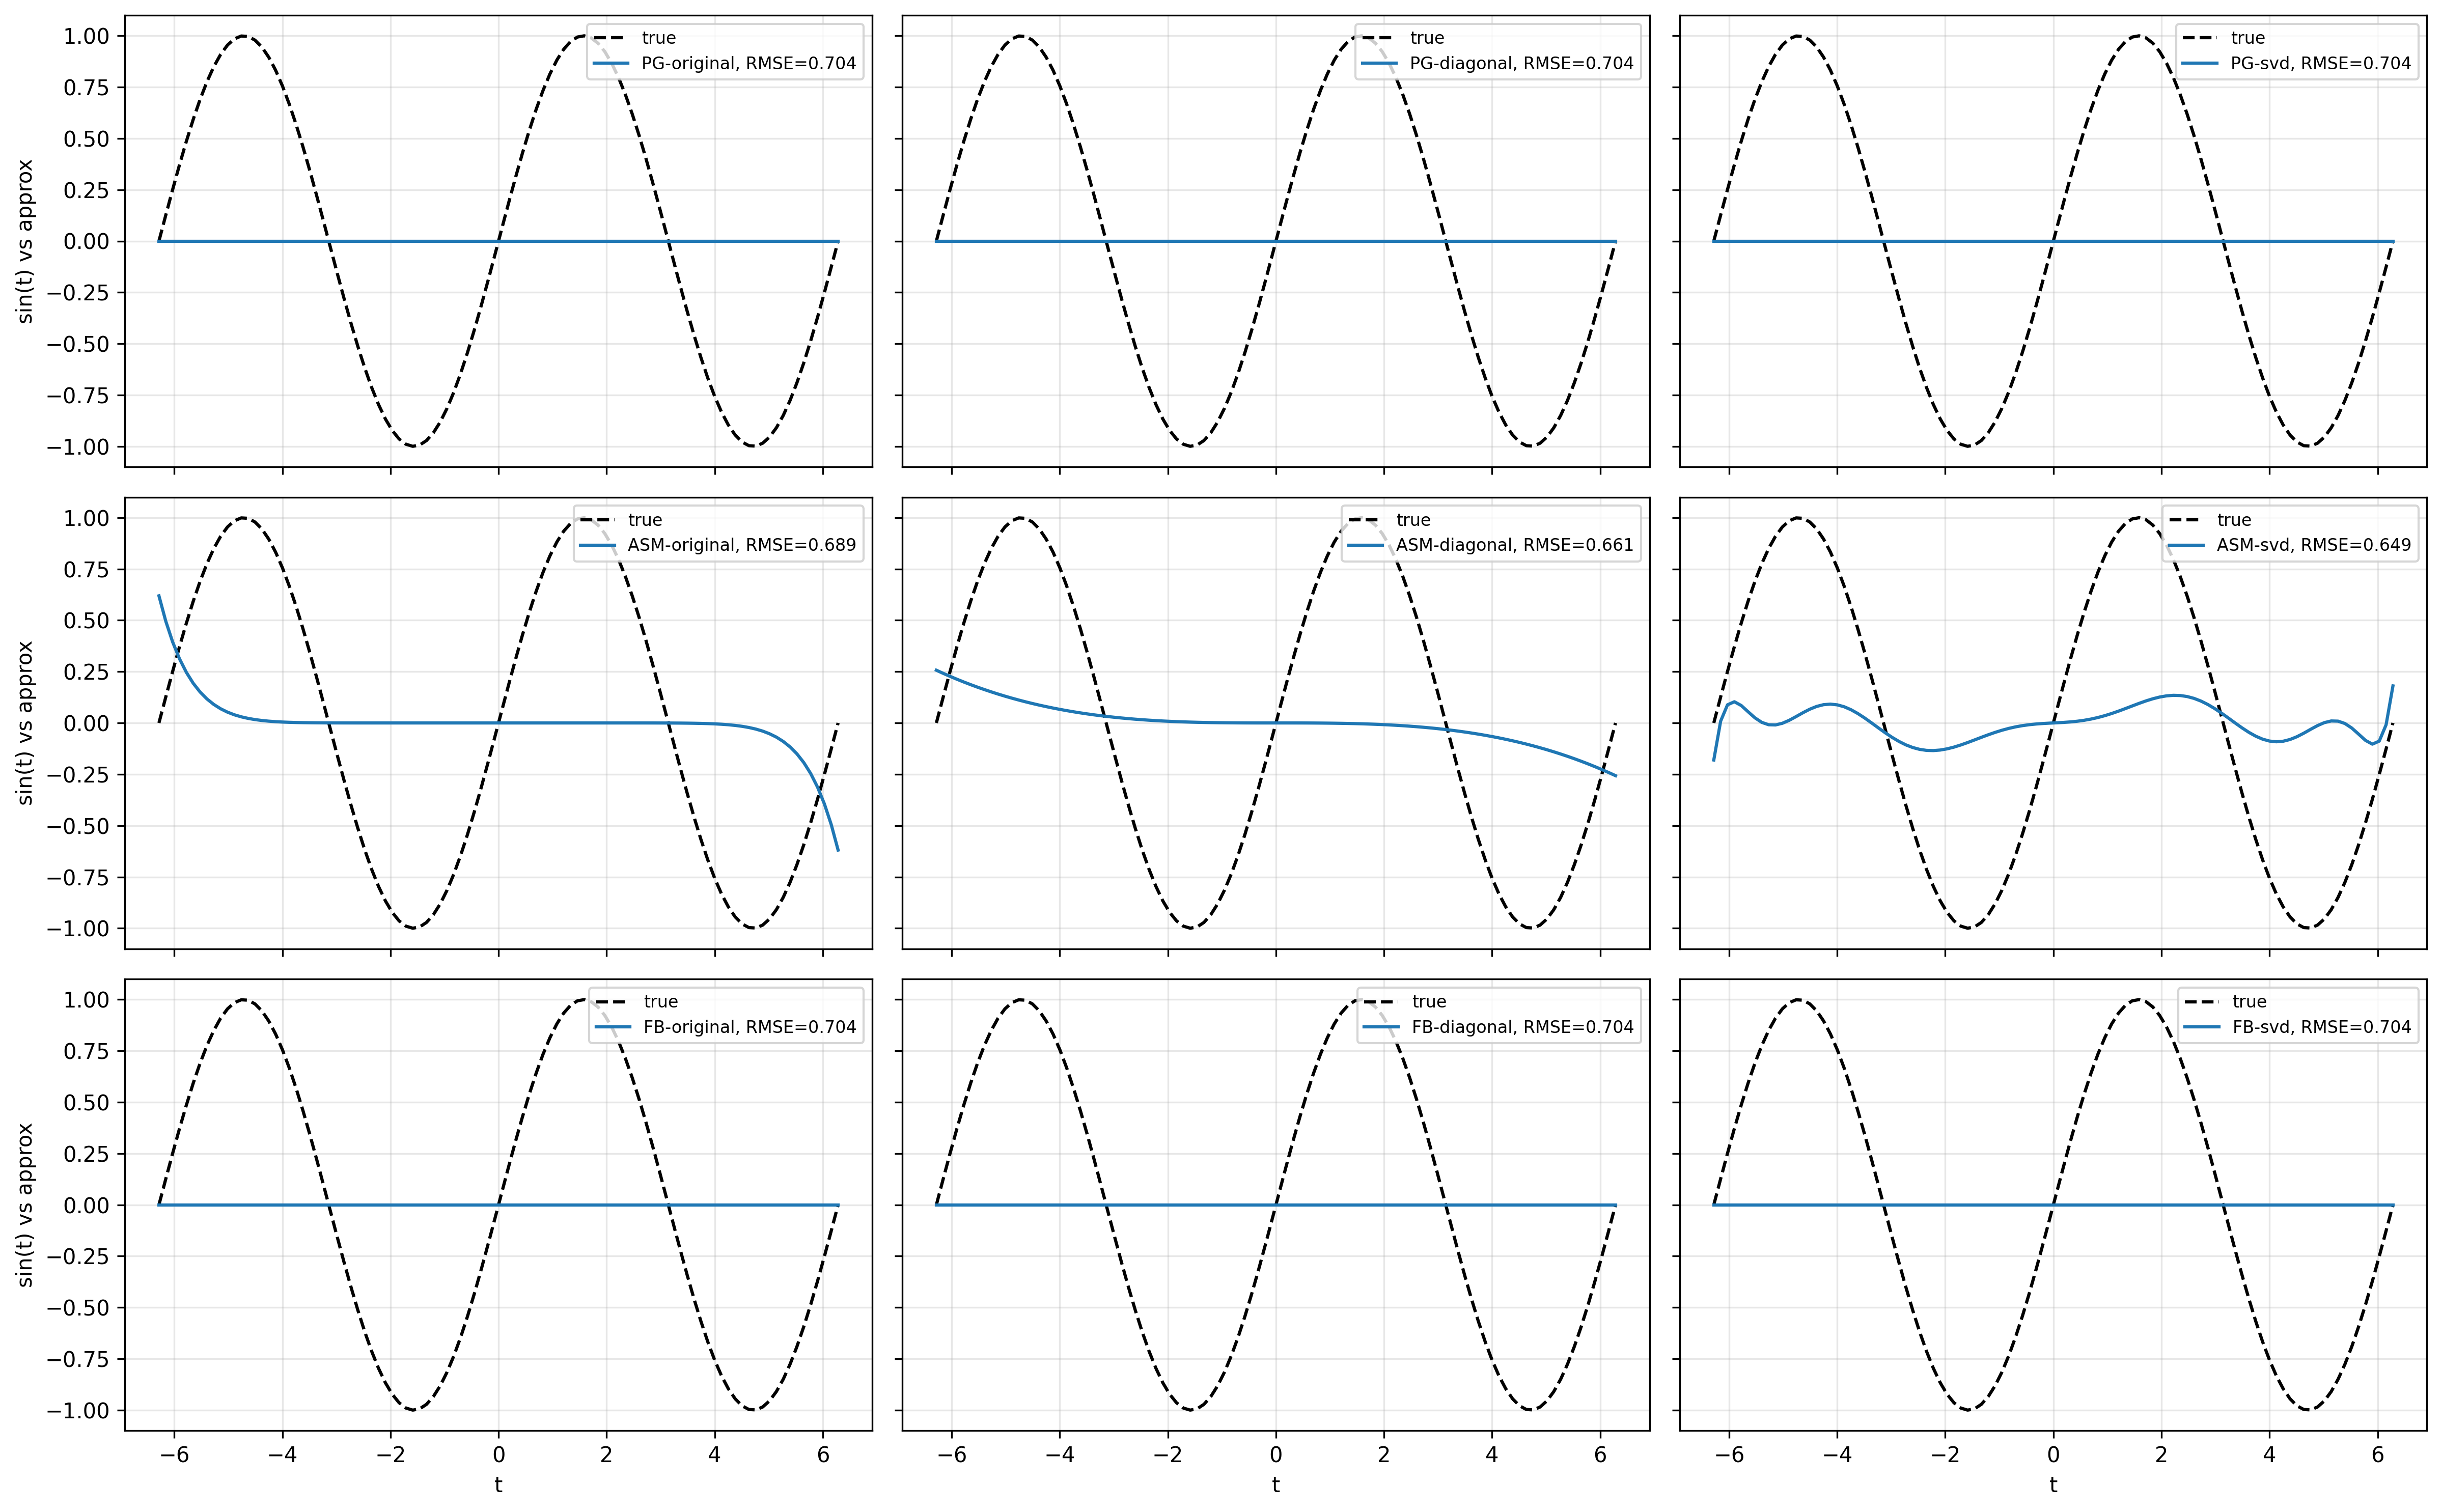
\includegraphics[width=\textwidth]{../results/plots/task4_approximation_quality.png}
\caption{Task 4 Approximation Quality (Degree 12): Best per algorithm and method; pre-conditioning improves fit quality and stability.}
\label{fig:task4_quality}
\end{figure}

\subsection{Discussion}
\begin{itemize}
    \item \textbf{Trade-off}: SVD delivers maximal conditioning (and performance) but with higher pre-processing cost; diagonal is a robust default.
    \item \textbf{Algorithm sensitivity}: ASM benefits notably from pre-conditioning; PG and FB also improve but are bounded by the feasible set/regularization.
    \item \textbf{Recommendation}: Use diagonal pre-conditioning in practice; consider SVD for small-to-medium $n$ when setup time is acceptable.
\end{itemize}

\subsection{Reproducibility}
Task 4 data and plots are saved as:
\begin{itemize}
    \item \textbf{Data}: \texttt{results/data/task4\_results.pkl}, \texttt{results/data/task4\_results.json}
    \item \textbf{Plots}: \texttt{results/plots/task4\_preconditioned\_performance.png}, \texttt{results/plots/task4\_approximation\_quality.png}
\end{itemize}

The data includes:
\begin{itemize}
    \item Complete solution vectors and convergence histories
    \item Performance metrics (iterations, objective values, optimality measures)
    \item Problem parameters and condition numbers
    \item Algorithm-specific results and comparisons
\end{itemize}

\end{document}
